%%%%%%%%%%%%%%%%%%%%%%% file template.tex %%%%%%%%%%%%%%%%%%%%%%%%%
%
% This is a general template file for the LaTeX package SVJour3
% for Springer journals.          Springer Heidelberg 2010/09/16
%
% Copy it to a new file with a new name and use it as the basis
% for your article. Delete % signs as needed.
%
% This template includes a few options for different layouts and
% content for various journals. Please consult a previous issue of
% your journal as needed.
%
%%%%%%%%%%%%%%%%%%%%%%%%%%%%%%%%%%%%%%%%%%%%%%%%%%%%%%%%%%%%%%%%%%%
%

\RequirePackage{fix-cm}
%
%\documentclass{svjour3}                     % onecolumn (standard format)
%\documentclass[smallcondensed]{svjour3}     % onecolumn (ditto)
\documentclass[smallextended, natbib]{svjour3}       % onecolumn (second format)
%\documentclass[twocolumn]{svjour3}          % twocolumn
%
\smartqed  % flush right qed marks, e.g. at end of proof
%
\usepackage{graphicx}

%https://www.overleaf.com/project/5d93fcd4f993680001c5ae75
% \usepackage{mathptmx}      % use Times fonts if available on your TeX system
%
% insert here the call for the packages your document requires
%\usepackage{latexsym}
%\usepackage{amsmath}
\usepackage{float}
\usepackage{url}
\usepackage{mathpazo}    % to use Palatino font
\usepackage{amsmath}
%\usepackage{subcaption}
\usepackage{setspace}
\usepackage{pythonhighlight}
\usepackage{hyperref}

\onehalfspacing 
%
% please place your own definitions here and don't use \def but
% \newcommand{}{}
%
% Insert the name of "your journal" with
% \journalname{myjournal}
%

% To eliminate the header box activate the following
\def\makeheadbox{\relax}

\AtBeginDocument{%
  \paperwidth=\dimexpr
    1in + \oddsidemargin
    + \textwidth
    % + \marginparsep + \marginparwidth
    + 1in + \oddsidemargin
  \relax
  \paperheight=\dimexpr
    1in + \topmargin
    + \headheight + \headsep
    + \textheight
    % + \footskip
    + 1in + \topmargin
  \relax
  \usepackage[pass]{geometry}\relax
}

% Minimize hyphenation
\tolerance=1
\emergencystretch=\maxdimen
\hyphenpenalty=10000
\hbadness=10000


\begin{document}

\title{Spatial Heterogeneity Modeling for Regional Economic Analysis: 
}
\subtitle{A Computational Approach Using Python and Cloud Computing}



\author{Carlos Mendez$^a$ \and Qian Jiang$^a$
}

\providecommand{\JELkeywords}[1]{\textbf{JEL Classifications} #1}


\titlerunning{.} 
\authorrunning{.} % if too long for running head

\institute{
$^\alpha$ Graduate School of International Development, Nagoya University, Japan. \\
Carlos Mendez; \email{carlos@gsid.nagoya-u.ac.jp} \\
Qian Jiang; \email{akane.kyou777@gmail.com}
}

\date{(Version-20251104)}
% The correct dates will be entered by the editor


\maketitle

\begin{abstract}
\begin{singlespace}

Spatial heterogeneity modeling extends traditional regression analysis by identifying geographical variations in regression coefficients. It addresses the limitations of non-spatial models that assume spatial homogeneity in statistical relationships. This chapter introduces two methods for modeling spatial heterogeneity: Geographically Weighted Regression (GWR) and Multiscale Geographically Weighted Regression (MGWR). We illustrate their application in the study of regional income convergence in Indonesia.  Unlike classical convergence models that focus on a single convergence speed, a heterogeneous convergence approach provides a more nuanced understanding of regional processes by identifying the location multiple convergence clusters. This chapter also provides a comprehensive guide on implementing GWR and MGWR models using open source software and cloud computing. Specifically, it shows how to apply advanced Python libraries for geospatial analysis. It integrates real-world data from recent studies to clarify essential concepts. It employs Google Colab as a cloud-based computational environment to facilitate hands-on learning. This modern computational approach enables the reader to replicate and extend the analyses presented in the chapter, fostering a deeper understanding of spatial heterogeneity modeling.


% Extended abstract: 
% Spatially heterogeneity modeling is a spatial analysis technique that extends traditional regression models by incorporating local variations in parameter estimates across a geographical space. This approach addresses a critical limitation of conventional non-spatial regression models, which assume spatial homogeneity and overlook the inherent spatial heterogeneity in regional data. This chapter introduces methods for modeling spatial heterogeneity using both the classical Geographically Weighted Regression (GWR) and the newly developed Multiscale Geographically Weighted Regression (MGWR) framework. We present foundational concepts and applications of spatial heterogeneity modeling within the context of regional growth and development studies. In particular, the chapter showcases the application of GWR and MGWR models to understand the process of regional convergence in Indonesia, a country characterized by large economic disparities across its numerous islands and districts. Through this case study, we illustrate how spatial heterogeneity models can assess not only the direction and magnitude of convergence speed but also evaluate the location and scale of the convergence process. Unlike traditional non-spatial models that focus on a single average speed of convergence, the heterogeneous convergence approach identifies and analyzes various patterns of convergence beyond the average, allowing for a more nuanced understanding of regional dynamics. The chapter also offers a detailed presentation of the practical implementation of GWR and MGWR models, bridging the gap between theoretical concepts and real-world applications. By utilizing state-of-the-art Python libraries for geospatial modeling, incorporating real data applications from recent research, and leveraging a cloud-based computational environment, readers are provided with a hands-on learning experience. This approach enables them to replicate and extend the analyses presented in the chapter, fostering a deeper understanding of spatial heterogeneity modeling.

\end{singlespace}

\keywords{Spatial heterogeneity modeling \and Geographically Weighted Regression (GWR) \and Multiscale Geographically Weighted Regression (MGWR) \and Regional income convergence \and Open-source software \and Cloud computing}
\noindent
%\JELkeywords{O40 $\cdot$ O47 $\cdot$ R10 $\cdot$ R11}


\end{abstract}


\newpage

\section{Introduction}


Regional economic development exhibits inherent spatial heterogeneity, yet traditional regression modeling approaches often overlook this characteristic of regional data. 
Local economic conditions, institutional quality, and development trajectories can vary substantially across space, creating distinct patterns of growth and convergence that cannot be adequately captured by estimates of single or globally homogeneous parameters.
This spatial heterogeneity presents both a challenge and an opportunity for regional development studies \citep{Ingram2019, Mendez2022, mendez2025political}.

The limitations of conventional regression models in capturing spatial variations have motivated the development of more sophisticated analytical frameworks. 
Spatially heterogeneous modeling techniques, particularly Geographically Weighted Regression (GWR) and its extension, Multiscale Geographically Weighted Regression (MGWR), represent significant methodological advances in addressing these limitations. 
These approaches recognize that regression parameters can vary systematically across geographic space, allowing a more nuanced understanding of regional processes \citep{Brunsdon1996, Fotheringham2017, Fotheringham2023}.

The evolution from GWR to MGWR reflects a deeper understanding of spatial processes. 
Although GWR pioneered the concept of locally varying parameters, MGWR introduces the critical insight that different processes might operate at distinct spatial scales. 
This multiscale perspective is particularly relevant for regional development studies, where various economic forces ----from local market interactions to broader institutional frameworks ----influence growth patterns at different geographic scales.

Indonesia provides a compelling case study to illustrate these methodological advances. 
As the world's largest archipelagic state, Indonesia encompasses remarkable economic diversity across its more than 17,000 islands and 514 districts. 
This geographical fragmentation, combined with significant variations in economic development, creates a natural laboratory to study spatial heterogeneity in regional growth and convergence processes \citep{aginta2023regional, miranti2023social, santos2022regional}.
Furthermore, the unique spatial structure of the country allows us to examine how regional growth and convergence patterns vary not only in magnitude, but also in spatial scale.

In this context, this chapter introduces the application of spatial heterogeneity modeling via the GWR and MGWR frameworks.
First, it provides a brief overview of the theoretical framework for understanding spatial heterogeneity in regional development studies.
By contrasting traditional global models with GWR and MGWR approaches, we illustrate how spatial heterogeneity modeling can reveal local variations in regional growth and convergence patterns that would otherwise remain hidden.
Second, through an empirical application to Indonesian districts, we illustrate how these methods can identify distinct regional convergence clusters and their associated spatial scales. 
This analysis reveals patterns of convergence and divergence across different regions, challenging the assumption of a uniform convergence process. 
Third, we bridge the gap between theory and practice by providing detailed computational implementations using modern Python libraries for geospatial analysis.

Our quantitative approach leverages recent advances in computational methods and geospatial data availability. 
Using state-of-the-art Python libraries for geospatial modeling and a cloud computing platform, we demonstrate how spatial heterogeneity modeling techniques can be implemented efficiently and reproducibly. 
This cloud-based computational approach not only ensures the reliability of our results but also provides a template for future research in spatial heterogeneity modeling.

The remainder of this chapter is organized as follows. 
Section 2 presents a brief introduction to regional growth and convergence modeling. 
Section 3 introduces the foundations of spatial heterogeneity modeling, including the GWR and MGWR frameworks. 
The final section discusses implications for the analysis of regional development and offers directions for future research.


\section{Regional growth, development and convergence}

The study of regional economic growth and convergence represents one of the most important and enduring topics in development economics and regional science. 
Since the pioneering contributions of \cite{solow1956contribution} and later empirical investigations by \cite{barro1991economic} and \cite{barro1992convergence}, economists have sought to understand whether and under what conditions regional income disparities tend to diminish over time. 
This fundamental question has profound implications for regional development policy, as it determines whether market forces alone will eventually reduce spatial inequalities or whether targeted interventions are necessary to promote balanced regional development.

\subsection{Theoretical foundations: The neoclassical growth model}

To understand the concept of economic convergence, it is essential to begin with the theoretical foundations provided by the neoclassical growth model.
Originally developed by \cite{solow1956contribution}, the neoclassical growth model provides the theoretical framework that underlies most empirical convergence studies.
It also offers crucial insights into the mechanisms through which regional economies might converge over time.

The basic neoclassical growth model of Solow assumes that production in any economy is produced using a combination of capital ($K$), labor ($L$), and technology ($A$).
This conceptual notion is represented by a production function of the form $Y = F(K, AL)$, where $AL$ represents labor in efficiency units. 
Under the standard assumption of a Cobb-Douglas production function, it becomes $Y = K^\alpha (AL)^{1-\alpha}$, where $\alpha$ represents the capital share of output and lies between 0 and 1.

The model further assumes that a constant fraction $s$ of production is saved and invested, while capital depreciates at a rate $\delta$.
Both population and technology grow at exogenous rates $n$ and $g$, respectively. 
These assumptions lead to the fundamental dynamic equation that governs the evolution of capital per effective worker:
\begin{equation}
\dot{k} = sf(k) - (n + g + \delta)k,
\end{equation}
\noindent where $k = K/(AL)$ represents capital per effective worker and $f(k) = k^\alpha$ is the intensive form of the production function.

The key insight from this framework is that economies converge to a steady-state level of capital per effective worker, denoted $k^*$, where $sf(k^*) = (n + g + \delta)k^*$. 
At this steady state, all variables grow at their long-run rates.
Specifically, the production per worker grows at a rate $g$, while the level of output per worker depends on the fundamental parameters of the economy, including the savings rate, population growth, and technological progress.

The convergence prediction of the Solow growth model emerges from the diminishing returns to capital inherent in the production function. 
When an economy has low capital per worker relative to its steady state, the marginal product of capital is high, making investment attractive and driving rapid growth. 
In contrast, economies with high capital per worker face low marginal returns to capital, resulting in slower growth. 
This mechanism creates a natural tendency for poorer economies (those farther below their steady state) to grow faster than richer ones (those closer to their steady state), leading to convergence over time.

\subsection{Concepts of convergence: From theory to empirical testing}

The theoretical prediction of convergence from the Solow model has given rise to several empirical concepts. 
Researchers use various types of statistical tests to evaluate different concepts related to the original convergence prediction.
Understanding these different concepts is crucial for interpreting empirical results and designing appropriate testing frameworks.

\begin{itemize}
    \item \textbf{Absolute convergence} represents the strongest form of convergence and occurs when all economies converge to the same steady-state level of income per capita. This concept assumes that all regions or countries have identical fundamental characteristics, including savings rates, population growth rates, and access to technology. Under absolute convergence, initially poor regions should grow faster than initially rich ones, and income disparities should diminish over time without any conditioning variables. Empirically, absolute convergence can be tested by regressing growth rates on initial income levels and checking for a negative relationship.
    \item \textbf{Conditional convergence} provides a more nuanced and realistic framework that allows for differences in steady-state income levels across regions. This concept recognizes that regions may have different fundamental characteristics that affect their long-run income levels. Under conditional convergence, each region converges to its own steady state, which depends on region-specific factors such as institutions, geography, human capital, and policy environments. Empirically, conditional convergence is tested by including control variables that proxy for steady-state determinants alongside initial income in growth regressions.
    \item \textbf{Club convergence} represents an intermediate concept that allows the possibility that only groups of similar regions converge to common steady states. This concept emerged from theoretical work suggesting that economies with similar initial conditions and structural characteristics might converge to the same equilibrium, while different groups converge to different steady states. Club convergence is particularly relevant in spatial contexts, where geographic proximity might create similar institutional environments or technological spillovers that bind regions together in convergence clubs.    
\end{itemize}


The mathematical foundation for empirical convergence testing comes from linearizing the Solow model around its steady state. 
This linearization yields the convergence equation that forms the basis for most empirical work in this field. 
Starting from the dynamic equation for capital per effective worker and applying a Taylor expansion around the steady state, we can derive
\begin{equation}
\ln(y_{it}) - \ln(y_{i0}) = (1 - e^{-\gamma t})\ln(y_i^*) - (1 - e^{-\gamma t})\ln(y_{i0}),
\end{equation}

\noindent where $y_{it}$ is the income per capita at time $t$, $y_{i0}$ is the initial income per capita, $y_i^*$ is steady-state income per capita and $\gamma$ is the speed of convergence parameter. 
Rearranging this equation and dividing by $T$ gives us the following growth equation:
\begin{equation}
\frac{1}{T}[\ln(y_{iT}) - \ln(y_{i0})] = \frac{(1 - e^{-\gamma T})}{T}\ln(y_i^*) - \frac{(1 - e^{-\gamma T})}{T}\ln(y_{i0}), \label{eq:growth}
\end{equation}

\noindent where the growth rate $\frac{1}{T}[\ln(y_{iT}) - \ln(y_{i0})]$ is measured over the period 0 to $T$.

\subsection{The empirical convergence framework}

The analysis of regional economic growth and convergence has been a central theme in growth economics since the seminal works of \cite{barro1991economic} and \cite{barro1992convergence}.
The classical convergence hypothesis posits that poorer economies tend to grow faster than richer ones, leading to a long-run equilibrium where regional disparities diminish over time. 
This process can be empirically tested using a regression framework in which regional growth rates are explained by initial economic conditions.

Based on Equation \ref{eq:growth}, the standard growth and convergence model of \cite{barro1992convergence} can be expressed as

\begin{equation}
g(y)_{i,0-T}=\alpha - \frac{[1- e^{-\gamma T}]}{T} \cdot \log(y_{i0})+ \epsilon_{i},
\label{eq:betafull}
\end{equation}

\noindent where $g(y)_{i,0-T}$ represents the growth rate of region $i$ over the period 0 to $T$, $y_{i0}$ is the initial level of the economic variable under study, $\gamma$ captures the speed of convergence, and $\epsilon_i$ is the error term. For estimation purposes, this equation is commonly simplified to

\begin{equation}
g(y)_{i,0-T} = \alpha + \beta \cdot \log(y_{i0}) + \epsilon_{i},
\label{eq:betasimple}
\end{equation}

\noindent where $\beta$ is directly related to the convergence speed $\gamma$. 
A negative $\beta$ coefficient indicates convergence, as it implies that regions with lower initial development experience higher growth rates.

The coefficient $\beta$ in Equation \ref{eq:betasimple} has a direct economic interpretation. 
When $\beta < 0$, it indicates that regions with lower initial income levels tend to grow faster than those with higher initial income levels, consistent with the convergence hypothesis. 
The magnitude of $\beta$ is related to the speed of convergence through the relationship $\beta = -\frac{(1 - e^{-\gamma T})}{T}$, where $\gamma$ represents the underlying speed of convergence parameter from the theoretical model. 
A larger absolute value of $\beta$ indicates faster convergence, meaning that income gaps close more rapidly.

The economic intuition behind this relationship stems from the diminishing returns to capital in the neoclassical production function. 
Regions with low capital per worker (and thus low income) have high marginal products of capital, making investment particularly attractive and driving rapid growth. 
Conversely, regions with high capital per worker face diminishing returns, leading to slower growth rates. 
This mechanism creates an automatic tendency toward equalization of income levels over time.

\subsection{Limitations of traditional convergence models and the need for spatial approaches}

While the traditional convergence framework has provided valuable insights into regional growth patterns, it suffers from several important limitations that motivate the development of more sophisticated spatial approaches.
The most critical limitation is the assumption of parameter homogeneity across space.
Under this assumption, all regions follow the same convergence process with identical speed and steady-state characteristics.

This assumption of spatial homogeneity is increasingly recognized as unrealistic in the context of regional development. 
Different regions may face different institutional environments, infrastructure endowments, natural resource bases, and human capital stocks that fundamentally alter their growth trajectories. 
In addition, spatial spillovers, agglomeration effects, and geographic constraints can create locally varying growth dynamics that cannot be captured by traditional global regression approaches.

The assumption of independence across regional observations also becomes problematic when dealing with spatial data. 
Regions that are geographically close to each other often exhibit similar growth patterns due to shared technologies, common shocks, or economic spillovers. 
This spatial dependence violates the standard regression assumption of independent error terms and can lead to biased parameter estimates and invalid statistical inference.

Furthermore, the traditional approach treats all regions as following a single convergence process, potentially masking important heterogeneity in convergence patterns. 
Some regions might form convergence clubs that converge to similar steady states, while others might diverge or follow entirely different growth trajectories. 
These patterns of club convergence or spatial heterogeneity cannot be detected using conventional regression methods that impose parameter homogeneity.

Recognizing these limitations has led to the development of spatial econometric approaches.
More recently, spatial heterogeneity models such as Geographically Weighted Regression (GWR) and Multiscale Geographically Weighted Regression (MGWR) have allowed regression coefficients to vary smoothly across space.
This modeling approach enables researchers to identify local convergence clusters, detect spatial variations in convergence speeds, and account for the complex geographic dimensions of regional development processes.

\subsection{Regional development implications}

The choice between traditional global convergence models and local (spatial heterogeneity) approaches has profound implications for regional development policy. 
If convergence processes are spatially homogeneous, then uniform national policies might be appropriate and efficient.
However, if convergence exhibits spatial heterogeneity, with different regions following different growth trajectories and converging at different speeds, then place-based development strategies become essential.

Spatial heterogeneity in convergence patterns can arise from various sources, including differences in institutional quality, technological readiness, capital accumulation, and access to markets. 
Geographic factors such as natural resource endowments, coastal access, and topographic constraints can also create spatially varying growth dynamics. 
Moreover, agglomeration economies and spatial spillovers can generate self-reinforcing patterns of development that create persistent spatial inequalities.

In Application 1, we illustrate the process of regional convergence in the context of the districts of Indonesia. 
Based on the dataset of \cite{aginta2023regional}, we study economic growth performance of 514 districts over the 2010-2018 period. 
In particular, we are interested in testing the hypothesis that initially poor districts tend to grow faster than initially rich ones. However, as we will demonstrate through the application of the GWR and MGWR methods, this simple hypothesis masks considerable spatial heterogeneity in convergence patterns in Indonesia's diverse regional landscape.

The Indonesian case provides an ideal setting for examining spatial heterogeneity in convergence processes due to the country's remarkable geographic and economic diversity. 
As the world's largest archipelagic state, Indonesia encompasses thousands of islands with varying resource endowments, infrastructure connectivity, and institutional environments. 
This geographic fragmentation, combined with historical patterns of development that have favored certain regions over others, creates natural conditions for spatially heterogeneous growth and convergence processes.


\subsubsection*{Application 1: Regional growth and convergence in Indonesia}
% https://colab.research.google.com/drive/1Bsr20h4SX9F8TNiaLNO5eHNF5GI5jdps?usp=sharing
% URL: https://bit.ly/MGWRapp1

The code of Application 1 creates a scatterplot with a regression line to visualize the relationship between the initial (log) GDP per capita and its subsequent growth rate.
It begins by performing linear regression using the \verb|stats.linregress| function on the logarithm of GDP per capita in 2010 and the GDP growth rate over the 2010-2018 period. 
The code then calculates the R-squared value and sets up a figure using the \verb|matplotlib| and \verb|seaborn| libraries. 
A scatterplot with a regression line is created using \verb|sns.regplot|, with customized appearance settings for both the scatter points and the regression line. 
The plot is further customized by removing spines, adding labeled axes, and including a text box in the upper right corner that displays the convergence coefficient (with three stars to indicate statistical significance if $p < 0.01$) and the R-squared value. 
Finally, the layout is adjusted, the plot is saved as a PNG file, and then displayed. 

\begin{python}
##################################################################
# Application 1: Regional Growth and Convergence in Indonesia
# URL: https://bit.ly/MGWRapp1
##################################################################

# 1. Perform Linear Regression Analysis
# -------------------------------------
# Compute the relationship between log GDP per capita (2010)  
# and GDP growth rate (2010-2018).

slope, intercept, r_value, p_value, std_err = stats.linregress(
    gdf["ln_gdppc2010"], gdf["g"]
)

# Compute R-squared for goodness of fit
r_squared = r_value**2

# 2. Create Scatterplot with Regression Line
# ------------------------------------------
plt.figure(figsize=(12, 8))  # Set figure size
sns.set_style("whitegrid")   # Apply grid style

# Scatter plot with regression line
ax = sns.regplot(
    x="ln_gdppc2010", y="g", data=gdf,
    scatter_kws={"alpha": 0.5, "color": "navy", "s": 80},  
    line_kws={"color": "orange"}  
)

# Remove plot spines
sns.despine(left=True, bottom=True)

# 3. Customize Labels and Annotations
# -----------------------------------
plt.xlabel("Log GDP per capita (2010)", fontsize=16)  
plt.ylabel("GDP Growth Rate (2010-2018)", fontsize=16)  

# Highlight significant coefficients (p < 0.01)
coefficient_text = f"{slope:.2f}{'***' if p_value < 0.01 else ''}"

# Add regression stats box in upper-right corner
plt.text(
    0.95, 0.95,  # Position in axes coordinates  
    f"Convergence coefficient: {coefficient_text}\n"
    f"R-squared: {r_squared:.2f}",
    transform=plt.gca().transAxes, fontsize=16,  
    verticalalignment="top", horizontalalignment="right",
    bbox=dict(facecolor="white", edgecolor="gray", alpha=0.8)  
)

# 4. Improve Layout and Save Figure
# ---------------------------------
plt.tight_layout()  
plt.savefig("sc.png", dpi=150, bbox_inches="tight")  

# 5. Display the Plot
# -------------------
plt.show()  # Show plot

\end{python}

\begin{figure}[htbp]
    \centering
    \begin{minipage}{0.90\textwidth}
        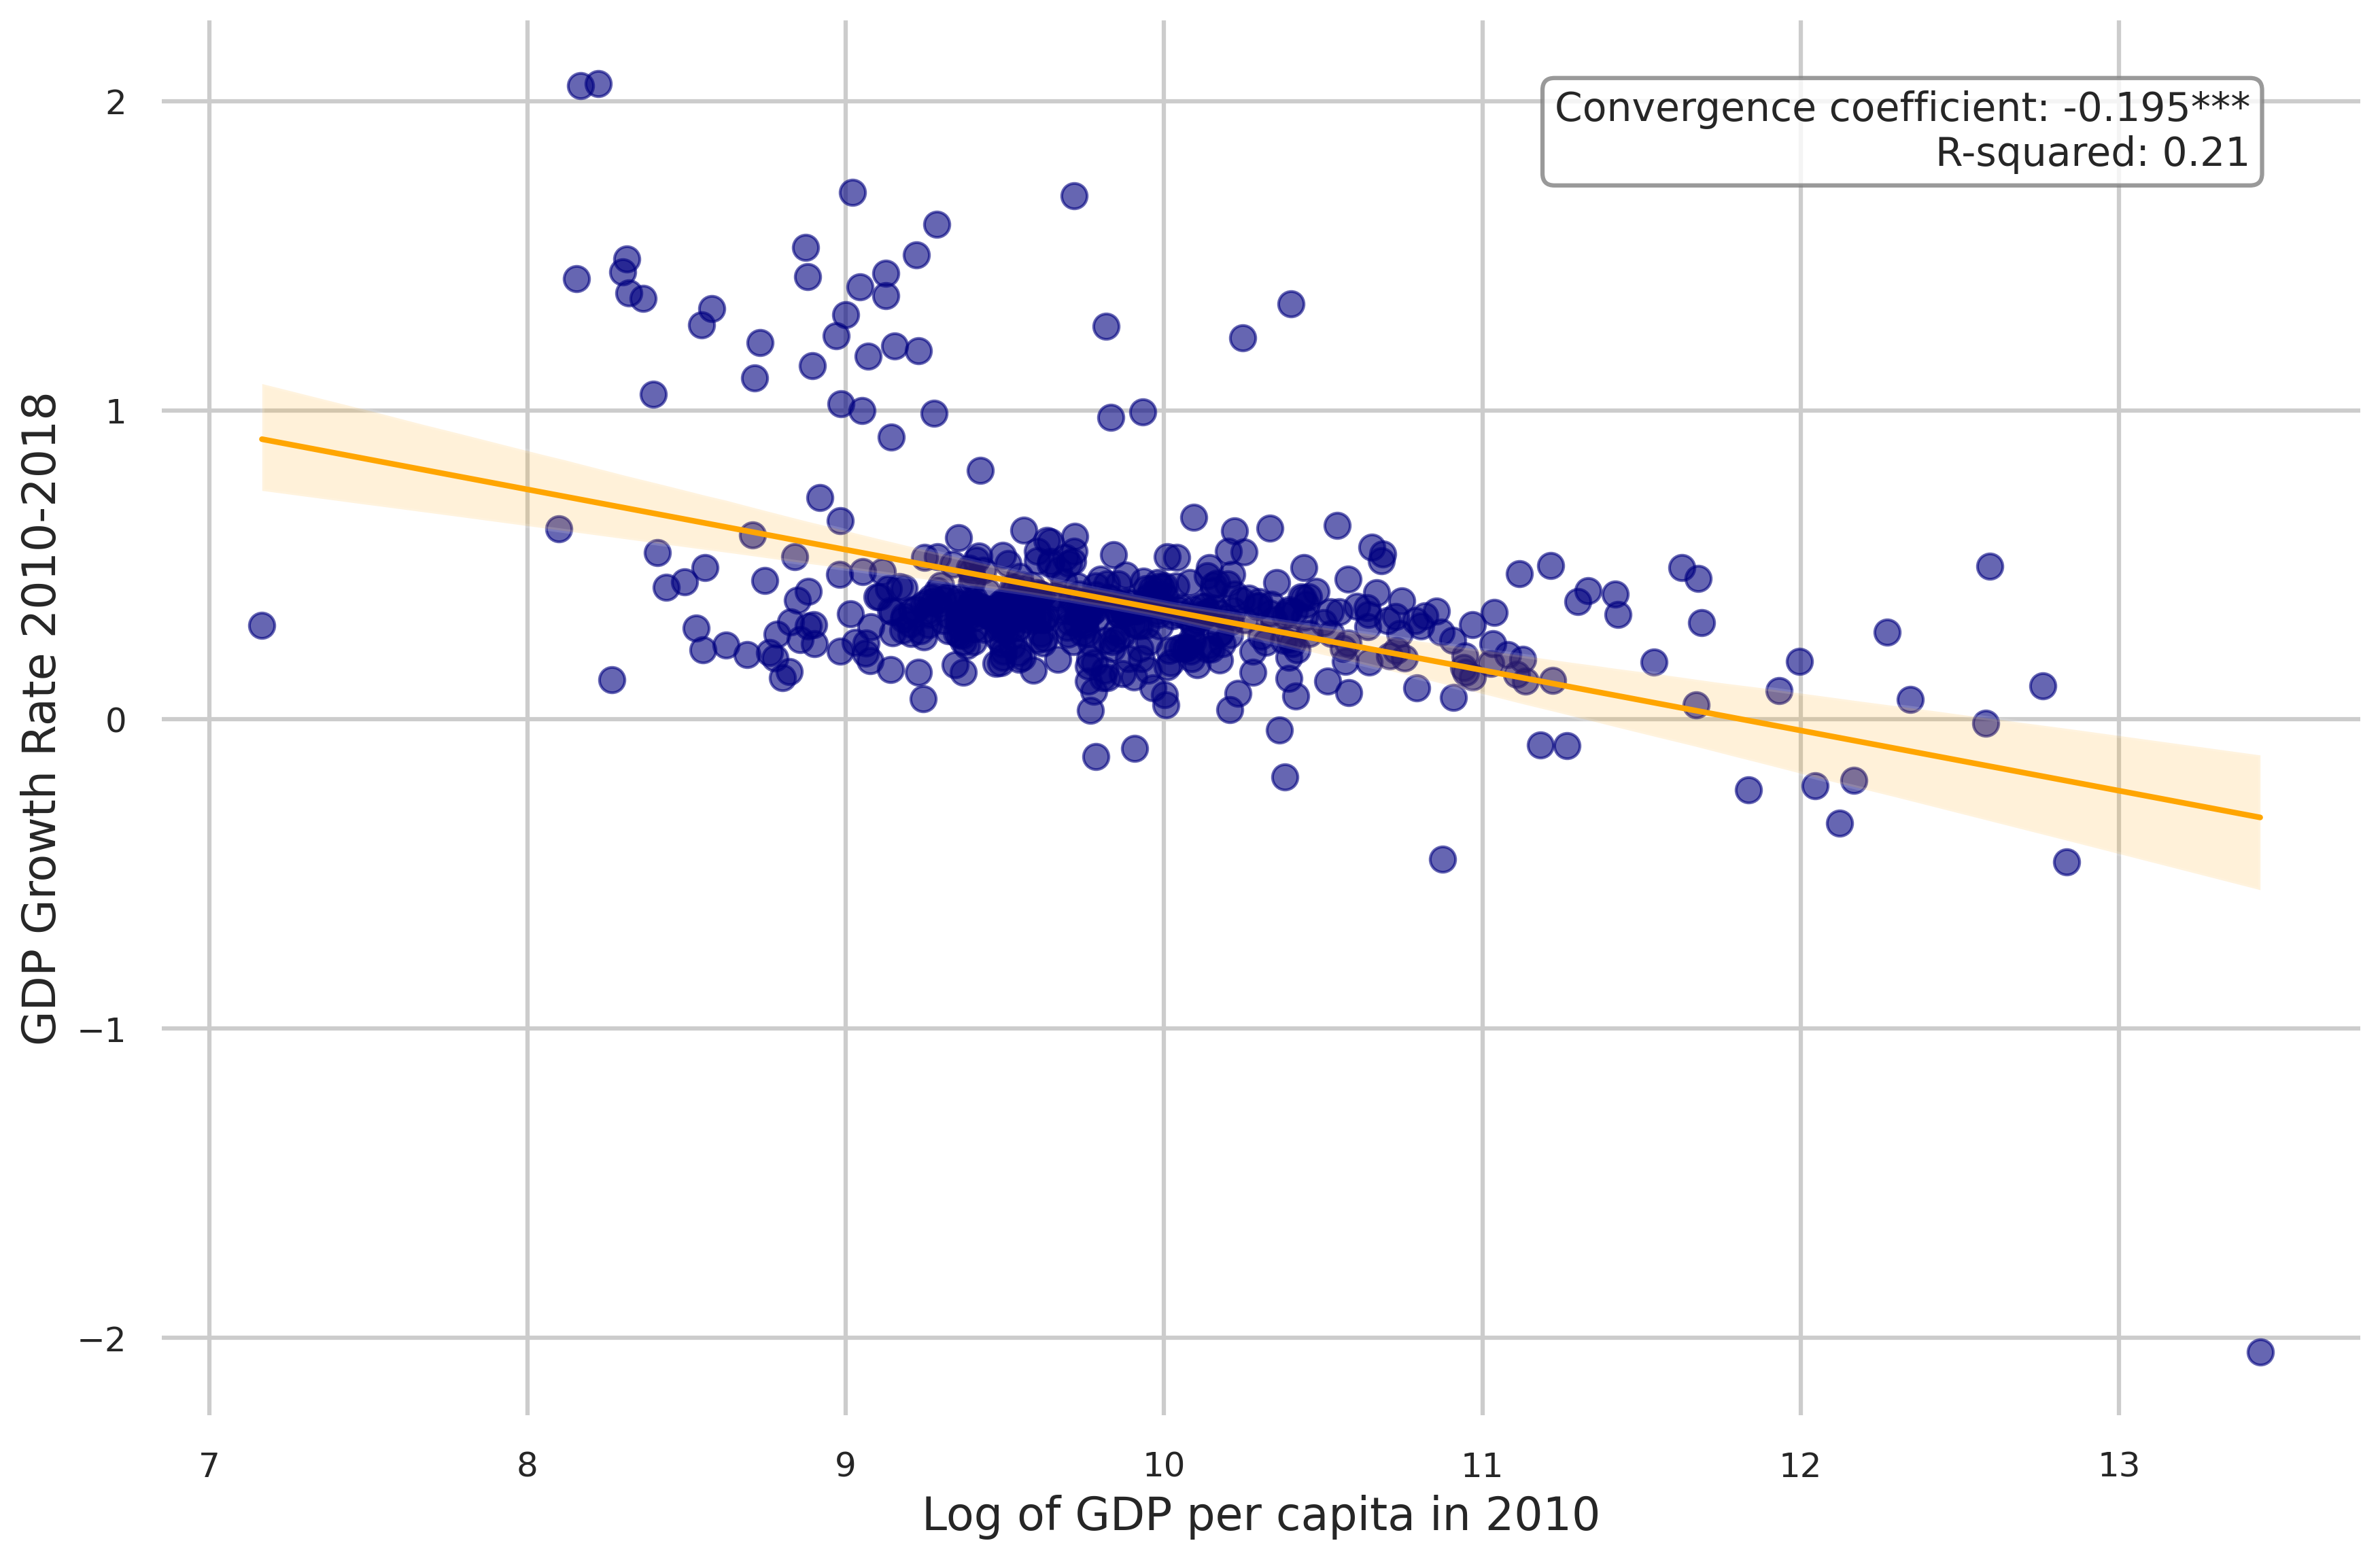
\includegraphics[width=\linewidth]{gdp_growth_scatter.png}
        \caption{Regional growth and convergence in Indonesia}
        \label{fig:gdp_growth_scatter}
    \end{minipage}
\end{figure}

Based on the code of Application 1, Figure \ref{fig:gdp_growth_scatter}  illustrates the relationship between initial economic conditions and subsequent growth across Indonesian districts. 
The x-axis shows the log of GDP per capita in 2010, while the y-axis displays the GDP growth rate from 2010 to 2018. 
Each blue dot represents a district, with the scatter demonstrating considerable variation in both initial GDP and growth rates. 
The downward trend line suggests a negative correlation between initial GDP and growth, indicating a pattern of economic convergence in which poorer districts tend to grow faster.
This relationship is quantified by a convergence coefficient of -0.195 (statistically significant) and an R-squared of 0.21. 
While this trend implies some degree of catch-up by less developed districts, the wide dispersion of data points and the modest R-squared value suggest that regional heterogeneity can be a phenomenon worth exploring.\footnote{See \cite{gunawan2021provincial}, \cite{mendez2020regional},  \cite{mendez2021disparities}, \cite{miranti2023social},  and \cite{santos2022regional} for alternatives approaches to study regional convergence and heterogeneity in the context of the Indonesian regions.} 


\section{Exploring and modeling spatial heterogeneity}


\subsection{Exploring spatial heterogeneity with choropleth maps}

Visualizing spatial patterns is crucial for understanding the complex geographic dimensions of economic phenomena, particularly in regional development studies.
Choropleth maps emerge as a critical tool for a preliminary exploration of spatial heterogeneity, offering an intuitive representation of how phenomena vary across geographic space.
The effectiveness of choropleth maps lies in their ability to transform abstract statistical data into a visual narrative that immediately reveals spatial patterns, clusters, and outliers.
Moreover, the Fisher Jenks algorithm can sharpen this visualization by optimizing the natural groupings within the data. 
This approach minimizes within-group variance while maximizing between-group variance, ensuring that the map reveals meaningful spatial patterns rather than arbitrary divisions. 
The algorithm's mathematical optimization produces classification breaks that correspond to inherent data structures, making it particularly valuable for identifying natural thresholds in economic indicators such as income levels, growth rates, or convergence coefficients.
As highlighted in the spatial modeling literature, such visualization techniques are not merely decorative but serve as powerful analytical tools that can help identify regional disparities, convergence clusters, and spatially varying economic processes.

Creating effective choropleth maps requires careful attention to cartographic design principles that enhance both analytical rigor and visual communication.
The choice of color scheme represents a fundamental decision that can significantly influence map interpretation.
Diverging palettes such as \texttt{coolwarm} prove particularly effective for representing phenomena with meaningful midpoints, such as convergence coefficients that can be positive or negative.
Sequential color schemes work best for unidirectional variables like GDP per capita, while qualitative schemes suit categorical data.
Beyond color selection, the number of classes used in the classification scheme impacts the balance between detail preservation and pattern clarity.
While Fisher Jenks optimization provides data-driven class boundaries, researchers must still determine the appropriate number of classes based on the data distribution and intended message.
Additionally, incorporating statistical significance filtering into choropleth displays—by masking or differentially shading non-significant regions—prevents the misinterpretation of random spatial variation as meaningful patterns.
This practice, demonstrated in the MGWR and GWR coefficient mapping applications, represents a crucial advancement in responsible spatial data visualization.

Basemap images can further enhance the exploration of spatial patterns by providing critical geographic context that grounds the analysis in a recognizable spatial framework. 
Different types of basemaps---from street maps that highlight administrative boundaries to satellite imagery that reveals terrain and land use---can be strategically selected to complement the research question and data being analyzed.
The layering of basemaps requires technical consideration of coordinate reference systems, transparency levels, and rendering order to ensure that the thematic data remains visually prominent while benefiting from the contextual information.
Modern Python libraries such as \texttt{contextily} facilitate seamless integration of web-based tile services, enabling researchers to incorporate high-quality basemaps from providers such as CartoDB, OpenStreetMap, or satellite imagery sources.
In the context of regional economic studies, a terrain or satellite basemap might help explain spatial economic patterns by revealing geographic features that could influence economic development, such as mountain ranges, coastal regions, or urban-rural divides.

The integration of multiple map elements—--thematic data layers, basemaps, legends, and annotations---demands careful attention to visual hierarchy and cartographic balance.
Effective maps employ techniques such as edge effects (using subtle boundaries between regions), appropriate line weights, and strategic use of labels to guide the viewer's attention without overwhelming the primary data display.
The choice of basemap becomes an integral part of the research narrative, transforming raw statistical data into a rich, contextually grounded representation of spatial economic dynamics.
Furthermore, when creating map series for comparing different variables or time periods, maintaining consistent design elements—including classification schemes, color palettes, and geographic extents—ensures that viewers can accurately compare patterns across maps.
These cartographic considerations, combined with robust statistical methods like Fisher Jenks optimization and regional filtering, elevate choropleth mapping from a simple visualization technique to a more rigorous analytical tool for understanding spatial heterogeneity in regional development studies.


In Application 2, we introduce choropleth mapping using the key variables of the convergence equation.
Two key components characterize our visualization approach.
The first is the use of the Fisher and Jenks algorithm to optimize the natural grouping of the regions.
The second is the use of a basemap image to provide geographic context.

\subsubsection*{Application 2: Mapping the spatial distribution of initial GDP and growth}
% https://colab.research.google.com/drive/1xmbZY1ZraU58eE1e-UdJ7w11S2WlH-1M?usp=sharing
% https://bit.ly/MGWRapp2

The code of Application 2 creates a figure with two vertically stacked maps using popular Python libraries such as  \verb|matplotlib|, \verb|geopandas|, and \verb|contextily|. 
It first defines a \verb|create_map()| function that plots data on a given axis, adds \verb|CartoDB| basemaps, and sets the titles. 
The function is called twice to create two different maps: one showing the log of GDP per capita in 2010 and another showing GDP per capita growth from 2010-2018. 
The code uses a color scheme based on the Fisher and Jenks classification method and the \verb|coolwarm| colormap to visualize the data. 
It adds both a background basemap and a label basemap overlay to provide geographic context. 
Finally, it adjusts the layout, saves the figure as a PNG file, and displays the plot. 

\begin{python}
##################################################################
# Application 2: Spatial Distribution of Initial GDP and Growth
# URL: https://bit.ly/MGWRapp2
##################################################################

# 1. Initialize Figure and Subplots
# ---------------------------------
fig, axes = plt.subplots(nrows=2, ncols=1, figsize=(12, 8))

# 2. Define Function to Create Map
# --------------------------------
def create_map(ax, data, column, title):
    # Plot spatial data with FisherJenks classification
    data.plot(
        column=column,
        scheme="FisherJenks",
        cmap="coolwarm",
        edgecolor="darkgrey",
        legend=True,
        ax=ax,
    )
    
    # Add base layers for geographic context
    cx.add_basemap(
        ax=ax,
        crs=data.crs.to_string(),
        source=cx.providers.CartoDB.Positron,
        attribution=False,
    )
    cx.add_basemap(
        ax=ax,
        crs=data.crs.to_string(),
        source=cx.providers.CartoDB.PositronOnlyLabels,
        attribution=False,
    )
    
    # Customize subplot appearance
    ax.axis("off")
    ax.set_title(title, fontsize=16)

# 3. Create Maps for Each Variable
# -------------------------------
create_map(
    ax=axes[0],
    data=gdf,
    column="ln_gdppc2010",
    title="(a) Log of GDP per capita in 2010"
)

create_map(
    ax=axes[1],
    data=gdf,
    column="g",
    title="(b) Growth of GDP per capita (2010-2018)"
)

# 4. Optimize Layout and Save Figure
# ----------------------------------
plt.tight_layout()
plt.savefig("map_xy.png", dpi=150, bbox_inches="tight")
plt.show()

\end{python}

\begin{figure}[htbp]
    \centering
    \begin{minipage}{0.99\textwidth}
        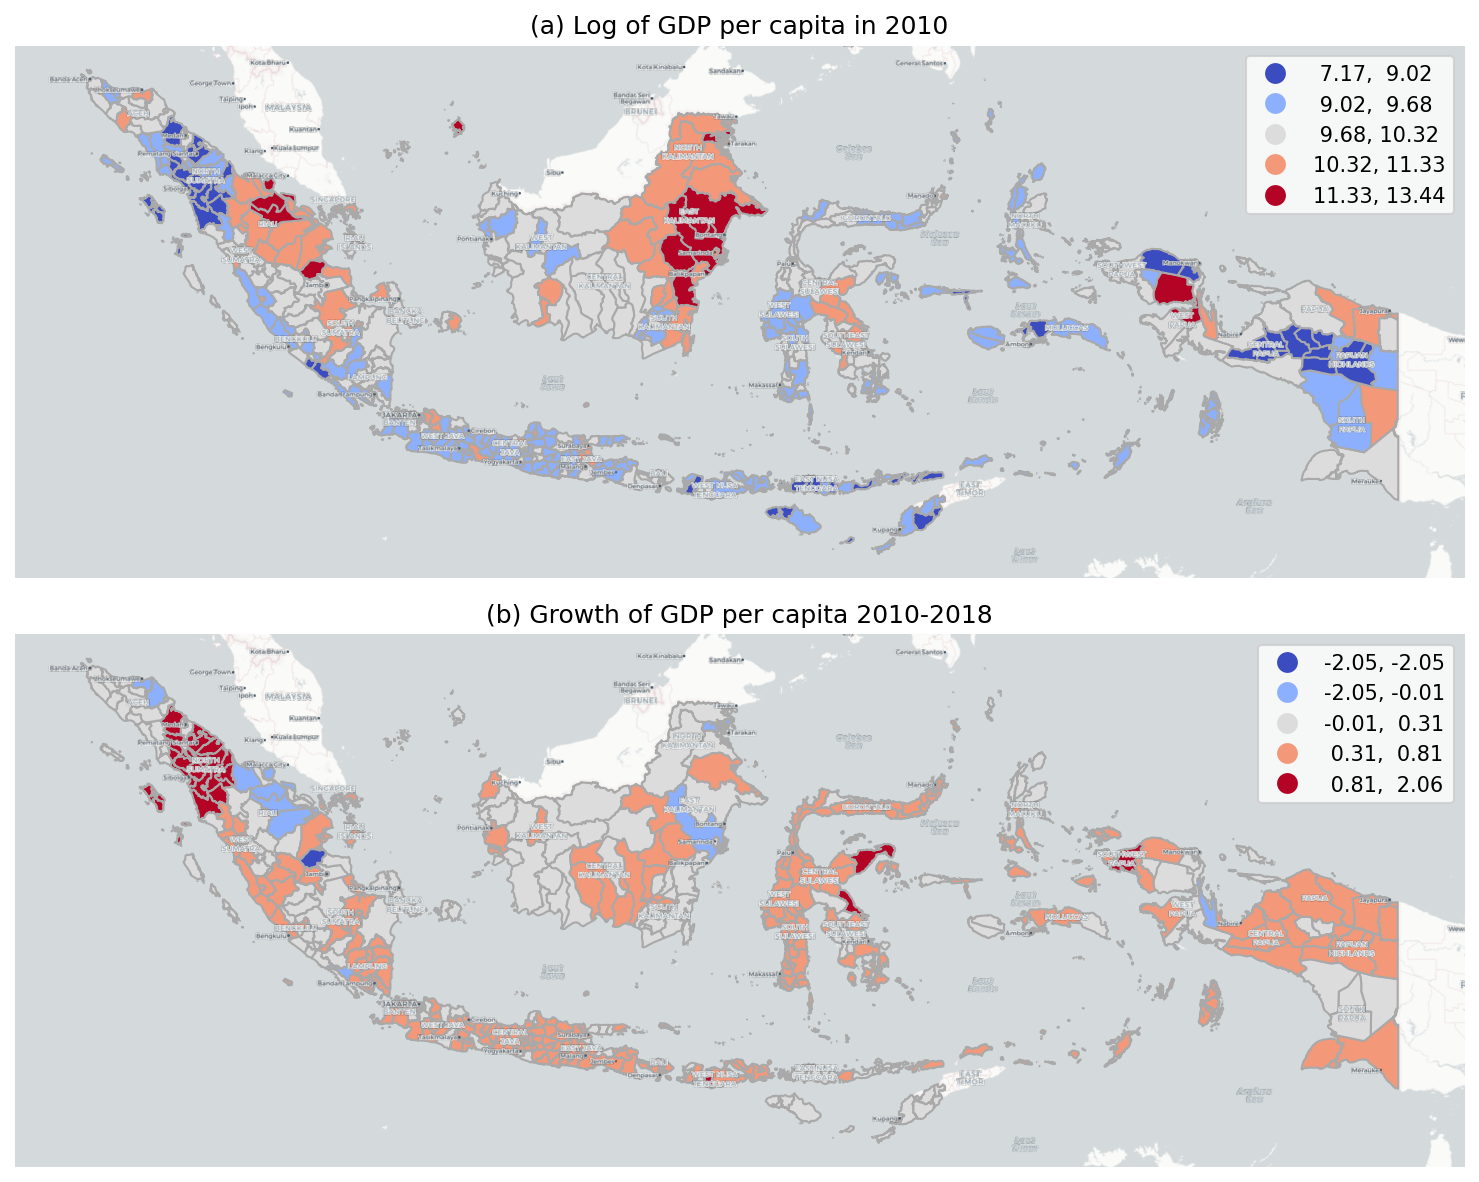
\includegraphics[width=\linewidth]{map_xy.png}
        \caption{Spatial distribution of initial GDP and growth}
        \label{fig:map_xy}
    \end{minipage}

\end{figure}

Based on the code of Application 2, Figure \ref{fig:map_xy} presents two maps of Indonesia.
The top map (a) shows the log of GDP per capita in 2010, using a color scale from dark blue (lowest values) to dark red (highest values). 
It reveals significant economic disparities, with eastern regions like Papua generally having lower GDP per capita, while Java and parts of Sumatra show higher values. 
The bottom map (b) depicts the growth of GDP per capita from 2010 to 2018, with colors ranging from dark blue (negative growth) to dark red (highest growth). 
Most of Indonesia experienced positive growth during this period.
Figure \ref{fig:map_xy} also illustrates the  inverse relationship between initial conditions and GDP growth.
Together, these maps provide an initial exploratory view of Indonesia's economic and geographical landscapes. highlighting regional variations in initial levels development and subsequent growth rates.


\subsection{Modeling spatial heterogeneity}

\subsubsection{Geographically weighted regression}

The limitations of global regression models become apparent when examining regional economic phenomena, where the assumption of spatial homogeneity often fails to capture the complex realities of geographic variation. 
Consider the relationship between education and economic growth.
While a global model might suggest a uniform positive effect across all regions, the actual impact likely varies substantially based on local industrial structures, institutional quality, and technological infrastructure. 
In Silicon Valley, for example, an additional year of education might yield dramatically different returns compared to rural agricultural regions. 
This spatial heterogeneity in regression coefficients represents a fundamental challenge that standard global  models cannot address.

Global regression models, by their very design, produce single-parameter estimates that represent average relationships across an entire study area. 
This averaging process obscures potentially important local variations and can lead to misleading policy recommendations. 
For example, when a global model reports that infrastructure investment increases regional GDP by 2\%, this masks the reality that the effect might be 5\% in landlocked regions desperate for connectivity and near zero in already well-connected coastal areas. 
Such spatial averaging not only reduces explanatory power, but also fails to identify regions where targeted interventions would be most effective.

The inadequacy of global models extends beyond simple parameter heterogeneity. 
Spatial data often exhibit complex patterns of local clustering, regional trends, and scale-dependent processes that violate the fundamental assumptions of ordinary least squares regressions.
The resulting spatial autocorrelation in the regression residuals indicates a misspecification of the model.
Thus, important spatial structures remain uncaptured. 
Moreover, global models implicitly assume that the processes generating observed outcomes operate uniformly across space.
This assumption of spatial homogeneity is increasingly challenged by empirical evidence that shows that economic, social, and environmental processes are inherently location dependent \citep{anselin1988spatial}.

Geographically Weighted Regression (GWR) emerges as a powerful alternative that explicitly acknowledges spatial heterogeneity in statistical relationships. 
Rather than estimating a single set of regression coefficients, GWR produces location-specific regression coefficients that can continuously vary over space. 
This local modeling approach aligns with the fundamental geographic principle that nearby locations tend to be more similar than distant ones, while still allowing for spatial variation in the strength of the relationships \citep{tobler1970computer}.

The superiority of local regression in capturing spatial heterogeneity manifests itself through several mechanisms. 
First, it allows different factors (covariates) to dominate in different regions. 
As such, it reflects the reality that regional economies operate under varying constraints and opportunities. 
Second, it captures changes in spatial regimes, where relationships might fundamentally differ across boundaries, be they administrative, cultural, or economic. 
Third, it provides a more nuanced understanding of spatial processes by revealing not just where outcomes differ, but why they potentially differ through spatially varying parameter estimates.

\subsubsection*{Historical development and foundations}

The development of GWR can be traced through several intellectual lines in statistics.
The expansion method, introduced by \cite{casetti1972generating}, provided an early framework for allowing the parameters to vary as functions of other variables, including spatial coordinates. 
This approach recognized that regression coefficients might not be constant but could systematically vary with contextual factors. 
However, the expansion method required pre-specification of the functional form of parameter variation, limiting its flexibility in capturing complex spatial patterns.

The kernel regression literature in statistics, particularly the work of \cite{cleveland1979robust} on locally weighted regression (LOESS), provided crucial methodological foundations. 
These nonparametric approaches showed how local fitting could reveal patterns obscured by global models. 
The adaptation of these ideas to explicitly spatial contexts, where the kernel is defined over geographic space rather than attribute space, represents the key innovation of GWR.

The formal introduction of GWR by \cite{Brunsdon1996} synthesized these approaches into a coherent framework specifically designed for spatial data analysis. 
Their insight was that spatial coordinates provide a natural organizing principle for local regression, with geographic proximity serving as the basis for defining local subsets of data. 
This geographic focus distinguishes GWR from general kernel regression methods and aligns it with the fundamental principles of spatial analysis.

\subsubsection*{First law of geography, spatial weighting and kernel functions}

The foundation of GWR rests on the concept of spatial weighting, which operationalizes Tobler's First Law of Geography: "everything is related to everything else, but near things are more related than distant things" \citep{tobler1970computer}. 
This principle is implemented through kernel functions that assign weights to observations based on their proximity to each regression point. 
The weighting scheme ensures that nearby observations contribute more to local parameter estimation than distant ones, creating a spatially adaptive modeling framework.

The mathematical formulation of spatial weights involves two key components: a distance metric and a kernel function. 
The distance metric, typically the Euclidean distance for projected coordinates or the great circle distance for geographic coordinates, quantifies spatial separation. 
The kernel function transforms these distances into weights that decay with increasing separation. 
The rate of this spatial influence decay----controlled by the bandwidth parameter of the kernel----fundamentally determines the spatial scale of the analysis.

Kernel functions in GWR serve as the mathematical representation of spatial influence decay. 
The most commonly employed kernels include the Gaussian, exponential, and bi-square functions, each with distinct properties that affect model behavior. 
The Gaussian kernel, with its smooth decay function, assigns continuously decreasing weights with distance:
$$w_{ij} = \exp\left(-\frac{1}{2}\left(\frac{d_{ij}}{h}\right)^2\right),$$
where $w_{ij}$ represents the weight of observation $j$ for regression point $i$, $d_{ij}$ is the distance between locations, and $h$ is the bandwidth parameter controlling the rate of distance decay.

The smooth decay of the Gaussian kernel ensures differentiability, which can be advantageous for optimization procedures. 
However, it never reaches exactly zero, which means that even very distant observations retain some influence. 
In practice, weights become negligibly small beyond a certain distance, but this theoretical non-zero influence can have computational implications for large datasets.
The exponential kernel provides an alternative smooth weighting function with a different decay rate:
$$w_{ij} = \exp\left(-\frac{d_{ij}}{h}\right).$$
This kernel decays more slowly than the Gaussian near the regression point but more rapidly at greater distances. 
The choice between Gaussian and exponential kernels often depends on beliefs about how quickly spatial influence should decay.

The bi-square kernel, in contrast, enforces a hard threshold beyond which observations receive zero weight:
$$w_{ij} = \begin{cases}
\left(1 - \left(\frac{d_{ij}}{h}\right)^2\right)^2 & \text{if } d_{ij} < h \\
0 & \text{otherwise.}
\end{cases}$$
The bi-square kernel creates a more localized regression that completely excludes distant observations, potentially reducing computational burden while maintaining local focus. 
The compact support of the bisquare kernel makes it particularly suitable for situations where a clear spatial limit to influence is conceptually appropriate.

Recent research has explored adaptive kernel functions that adjust their shape based on the characteristics of local data \citep{wolf2018single}. 
These advanced kernels can provide more nuanced weighting schemes, but at the cost of increased complexity and computational demands.
The choice between fixed and adaptive bandwidths represents another crucial consideration. 
Fixed kernels use a constant distance bandwidth across all regression points, which can be problematic in areas with heterogeneous data density. 
In sparse regions, a fixed bandwidth might encompass too few observations for reliable estimation, while in dense areas, it might include so many observations that local variation is obscured.
Adaptive kernels, specified as the k-nearest neighbors, ensure consistent local sample sizes but allow the spatial extent of influence to vary. 
In regions with sparse data, the kernel expands to capture sufficient observations, while in data-rich areas it contracts to maintain local focus. 
This adaptability makes adaptive kernels particularly suitable for irregular point patterns common in socioeconomic data. 
The formal specification of an adaptive kernel modifies the weight calculation to use ranks instead of distances:
$$w_{ij} = f\left(\frac{r_{ij}}{k}\right)$$
where $r_{ij}$ is the rank of observation $j$ in terms of distance from $i$, and $k$ is the number of nearest neighbors.

\begin{figure}[htbp]
    \centering
    \begin{minipage}{0.85\textwidth}
        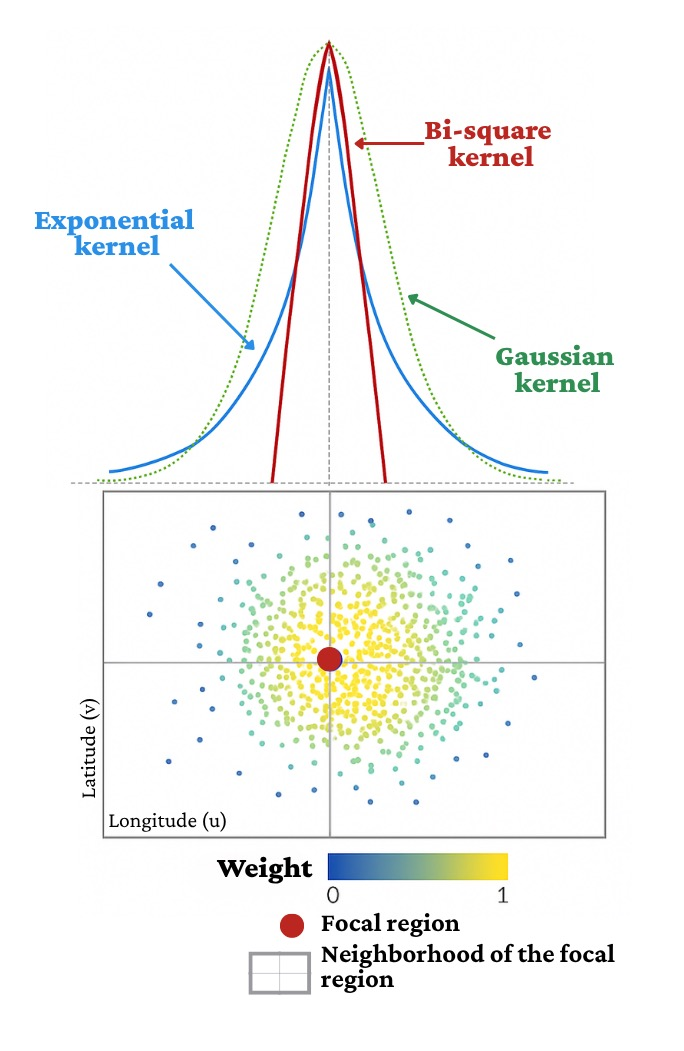
\includegraphics[width=\linewidth]{introGWRfigure.jpg}
        \caption{Spatial weights and kernel functions for heterogeneity modeling}
        \label{fig:introGWRfigure}
    \end{minipage}

\end{figure}

Figure \ref{fig:introGWRfigure} illustrates the fundamental weighting schemes that enable spatial heterogeneity modeling in geographically weighted regression models.
The three kernel functions (Gaussian, exponential,bi-square) represent different approaches to implementing Tobler's First Law of Geography.
Each kernel function determines how the influence of neighboring observations diminishes with distance from the focal region.
The bi-square kernel provides a sharp cutoff where weights reach exactly zero at the bandwidth threshold, effectively excluding distant observations from the local regression.
In contrast, Gaussian and exponential kernels allow all observations to retain some influence, albeit potentially very small, regardless of their distance from the regression point.

The spatial distribution of the weighted observations in the lower panel of Figure \ref{fig:introGWRfigure} illustrates how the kernel functions operationalize the concept of "borrowing data from nearby locations" that is central to the GWR methodology. 
The color gradient from blue (weight = 0) to yellow (weight = 1) visualizes how observations closer to the focal region receive higher weights in the local parameter estimation process. 
This weighting scheme addresses a fundamental challenge in spatial analysis: how to balance the need for sufficient data to estimate reliable local parameters while maintaining sensitivity to spatial variations in the underlying processes.
The rectangular boundary represents the neighborhood of the focal region, within which the kernel function determines the specific weight assigned to each observation. 
This approach enables the GWR to capture spatial heterogeneity by allowing regression coefficients to vary smoothly across a geographic space, with each local estimate informed primarily by nearby observations while accounting for the spatial structure of the data.


\subsubsection*{Bandwidth selection and spatial scale}


Bandwidth selection emerges as perhaps the most critical decision in spatial heterogeneity modeling.
The bandwidth of a kernel function controls the fundamental trade-off between bias and variance in local estimates. 
A bandwidth that is too small produces highly variable parameter estimates with large standard errors, while an excessively large bandwidth approaches the global model, failing to capture local variation.
The optimal bandwidth minimizes a model selection criterion that balances goodness-of-fit against model complexity.

The theoretical framework for bandwidth selection draws on the bias-variance decomposition of mean squared error. 
For a local estimator $\hat{\beta}_i$, the mean squared error can be expressed as:
$$MSE(\hat{\beta}_i) = \text{Bias}(\hat{\beta}_i) + \text{Var}(\hat{\beta}_i).$$
As the bandwidth decreases, the bias typically decreases (the estimate becomes more local) but variance increases (fewer observations contribute substantially). 

An optimal bandwidth aims to achieve the best compromise between the forces of bias and variance.
The method of Cross-validation (CV) provides an intuitive approach to bandwidth selection by evaluating predictive performance:
$$CV(h) = \sum_{i=1}^{n}(y_i - \hat{y}_{i(\neq i)})^2,$$
where $\hat{y}_{i(\neq i)}$ is the fitted value for observation $i$ when that observation is omitted from prediction.
This leave-one-out approach directly measures predictive accuracy but can be computationally intensive for large datasets.
Information criteria offer an alternative method that considers both fit and model complexity. 
The Akaike Information Criterion corrected for small samples (AICc) has become the standard choice:
$$AICc = 2n\ln(\hat{\sigma}) + n\ln(2\pi) + n\left(\frac{n + \text{tr}(\mathbf{S})}{n - 2 - \text{tr}(\mathbf{S})}\right),$$
where $\text{tr}(\mathbf{S})$ represents the trace of the hat matrix, serving as a measure of model complexity. 
The AICc penalizes models with many effective parameters, preventing overfitting that could arise from very small bandwidths.

Beyond its technical role in controlling the precision of the estimation, the bandwidth parameter also serves as an indicator of spatial scale in geographical processes. 
A small bandwidth reveals that the underlying relationship operates at a highly localized scale, suggesting that neighboring regions share similar characteristics only within narrow geographic bounds. 
In contrast, a large bandwidth indicates that spatial processes operate on broader spatial scales, where distant locations still exhibit similar characteristics in terms of estimated regression parameters. 
This interpretation transforms the notion of bandwidth from merely a statistical tuning parameter into a powerful tool for understanding spatial scale.
For example, the magnitude of the bandwidth can inform the geographic extent of economic spillovers, institutional influences, and development processes. 
In regional convergence studies, bandwidth estimates can provide suggestive evidence on whether convergence mechanisms operate through local agglomeration effects, broader regional policies, or national-level institutional frameworks.

\subsubsection*{Mathematical derivation: A brief overview}

The mathematical foundation of GWR extends that of the classical linear regression framework by incorporating the notion of spatial weights (and implicitly kernel function and bandwidth) into the derivation of the regression coefficients. 
Beginning with the standard global regression model in matrix notation:
$$\mathbf{y} = \mathbf{X}\boldsymbol{\beta} + \boldsymbol{\varepsilon},$$
where $\mathbf{y}$ is an $n \times 1$ vector of observations on the dependent variable, $\mathbf{X}$ is an $n \times k$ matrix of explanatory variables including the intercept, $\boldsymbol{\beta}$ is a $k \times 1$ vector of parameters, and $\boldsymbol{\varepsilon}$ is an $n \times 1$ vector of error terms with $E[\boldsymbol{\varepsilon}] = \mathbf{0}$ and $\text{Var}[\boldsymbol{\varepsilon}] = \sigma^2\mathbf{I}$.

GWR relaxes the assumption of parameter constancy by allowing parameters to vary as a function of location:
$$y_i = \sum_{j=1}^{k} \beta_j(u_i, v_i)x_{ij} + \varepsilon_i$$
where $(u_i, v_i)$ represents the coordinates of location $i$, and $\beta_j(u_i, v_i)$ is the value of the $j$th parameter at that location. 
This can be rewritten in matrix form for location $i$ as:
$$y_i = \mathbf{x}_i^T\boldsymbol{\beta}_i + \varepsilon_i$$
where $\mathbf{x}_i$ is a $k \times 1$ vector of explanatory variables at location $i$ and $\boldsymbol{\beta}_i$ is the corresponding parameter vector.

For each regression point $i$, we estimate a separate set of parameters using weighted least squares.
The objective function to minimize is:
$$Q_i = \sum_{j=1}^{n} w_{ij}(y_j - \mathbf{x}_j^T\boldsymbol{\beta}_i)^2$$
where $w_{ij}$ is the weight assigned to observation $j$ when calibrating the model at location $i$. Taking the derivative with respect to $\boldsymbol{\beta}_i$ and setting equal to zero:
$$\frac{\partial Q_i}{\partial \boldsymbol{\beta}_i} = -2\sum_{j=1}^{n} w_{ij}\mathbf{x}_j(y_j - \mathbf{x}_j^T\boldsymbol{\beta}_i) = \mathbf{0}$$
Solving for $\boldsymbol{\beta}_i$:
$$\sum_{j=1}^{n} w_{ij}\mathbf{x}_j\mathbf{x}_j^T\boldsymbol{\beta}_i = \sum_{j=1}^{n} w_{ij}\mathbf{x}_jy_j$$
In matrix notation, the parameter estimates at location $i$ are:
$$\hat{\boldsymbol{\beta}}_i = (\mathbf{X}^T\mathbf{W}_i\mathbf{X})^{-1}\mathbf{X}^T\mathbf{W}_i\mathbf{y}$$
where $\mathbf{W}_i$ is an $n \times n$ diagonal matrix with diagonal elements $w_{i1}, w_{i2}, \dots, w_{in}$, which represent the spatial weights described the previous section. 


\subsubsection*{Statistical properties and inference}

The statistical properties of GWR estimators differ fundamentally from those of the standard global regression. 
The local parameter estimates are biased but consistent under certain regularity conditions. 
The bias arises because each local regression uses data from nearby locations, where the true parameters may differ. 
As the sample size increases and the bandwidth adjusts appropriately, this bias diminishes.

The variance-covariance matrix for parameter estimates at location $i$ requires careful derivation. 
Under the assumption of homoscedastic errors:
$$\text{Var}(\hat{\boldsymbol{\beta}}_i|\mathbf{X}) = \sigma^2(\mathbf{X}^T\mathbf{W}_i\mathbf{X})^{-1}\mathbf{X}^T\mathbf{W}_i^2\mathbf{X}(\mathbf{X}^T\mathbf{W}_i\mathbf{X})^{-1},$$
this differs from the standard global regression case because $\mathbf{W}_i^2 \neq \mathbf{W}_i$ for the typical kernel functions.
The variance depends not only on the design matrix but also on the spatial configuration of the observations through the weight matrix.
For heteroscedastic errors, \cite{Brunsdon1996} propose a robust variance estimator:
$$\widehat{\text{Var}}_{\text{robust}}(\hat{\boldsymbol{\beta}}_i) = (\mathbf{X}^T\mathbf{W}_i\mathbf{X})^{-1}\mathbf{X}^T\mathbf{W}_i\hat{\mathbf{\Omega}}_i\mathbf{W}_i\mathbf{X}(\mathbf{X}^T\mathbf{W}_i\mathbf{X})^{-1},$$
where $\hat{\mathbf{\Omega}}_i$ is a diagonal matrix with elements $\hat{e}_j^2$, the squared residuals.

The effective number of parameters in GWR provides a measure of model complexity:
$$\text{ENP} = \text{tr}(\mathbf{S}).$$
This quantity varies between $k$ (the number of covariates, achieved when bandwidth is infinite) and $n$ (achieved when bandwidth approaches zero). 
The effective number of parameters plays a crucial role in model selection criteria and degrees of freedom calculations.

Hypothesis testing in GWR faces unique challenges due to the multiple testing problem and spatial dependence among test statistics.
\cite{DaSilva2016} developed corrections for multiple testing that account for the spatial structure of the tests. 
For testing the null hypothesis that a parameter is globally zero, they propose an adjusted significance level that depends on the effective number of parameters.
Testing for spatial variability in parameters represents another important inferential question. 
The null hypothesis that parameters are globally constant can be tested using Monte Carlo methods \citep{brunsdon1999some} or analytical approximations \citep{leung2000statistical}. 
These tests help determine whether the added complexity of GWR is justified by significant spatial variation in relationships.

\subsubsection*{Model diagnostics and validation}

Comprehensive model diagnostics are essential for validating the GWR results and identifying potential problems. 
Local collinearity diagnostics extend global measures to examine multicollinearity within each local regression \citep{wheeler2005multicollinearity}. 
The local condition number:
$$CN_i = \sqrt{\frac{\lambda_{\max}(\mathbf{X}^T\mathbf{W}_i\mathbf{X})}{\lambda_{\min}(\mathbf{X}^T\mathbf{W}_i\mathbf{X})}},$$
where $\lambda_{\max}$ and $\lambda_{\min}$ are the maximum and minimum eigenvalues, provides a measure of local multicollinearity. 
High condition numbers indicate potential instability in local parameter estimates.


Local measures of fit extend global $R^2$ to the local context:
$$R_i^2 = 1 - \frac{\sum_j w_{ij}(y_j - \hat{y}_j)^2}{\sum_j w_{ij}(y_j - \bar{y}_i)^2},$$
where $\bar{y}_i = \sum_j w_{ij}y_j / \sum_j w_{ij}$ is the locally weighted mean. 
These local $R^2$ values represent the proportion of variance explained by the local regression at each location, providing a spatially disaggregated view of model performance.  
The mapping of these local goodness-of-fit measures enables researchers to identify regions where the specified relationships adequately capture local dynamics versus areas where additional explanatory variables or alternative model specifications might be needed. 

Residual analysis in GWR must account for the complex structure induced by local fitting. 
Standardized residuals account for the varying leverage of observations:
$$r_i^{\text{std}} = \frac{e_i}{\hat{\sigma}\sqrt{1 - s_{ii}}}$$
where $s_{ii}$ is the $i$th diagonal element of the hat matrix. 
Mapping these standardized residuals can reveal areas of poor fit or model misspecification.



\subsubsection*{Some GWR applications in the study of regional convergence and development}

The application of GWR in regional science has revealed previously hidden spatial variations in economic relationships. 
Studies of regional convergence have shown that the speed and pattern of convergence vary substantially across space, challenging uniform policy prescriptions. .
Early empirical work, such as that conducted by \citet{eckey2006regional} on German regional convergence following reunification, indicated that convergence speeds appeared to vary between western and eastern areas. 
This spatial heterogeneity can potentially reflect structural differences in industrial composition, infrastructure quality, and institutional frameworks. 
This study criticized the conventional assumption in neoclassical growth models that regions converge at uniform rates towards a common equilibria.
Furthermore, it emphasized that place-specific factors might play a more significant role in shaping economic development trajectories than previously recognized.

Subsequent research has examined spatial heterogeneity across diverse countries, including Chinese urban centers \citep{li2007study}, European regional economies \citep{thissen2016competitive}, and United States metropolitan areas \citep{partridge2007geographic}. 
These studies have tended to reveal patterns of spatial variation in how development determinants operate across different geographic contexts.
For instance, in the case of China,  infrastructure investments are consistent with spatially different growth effects across Chinese regions. 
The evidence shows stronger impacts in inland areas compared to coastal regions. 
Similarly, evidence from European regions suggests that human capital investments exhibit varying returns depending on regional characteristics.
In particular, there is some indication of higher marginal returns in peripheral versus core metropolitan areas.
The United States context provides additional evidence into regional employment dynamics. 
\citet{partridge2007geographic} found that high-technology employment demonstrated spatially varying effects on overall employment growth across non-metropolitan areas. 
Their analysis suggested that technology-based employment had differential impacts depending on regional characteristics such as existing industrial structure, workforce education levels, and proximity to metropolitan centers. 

Recent research has begun to extend the analysis of spatial heterogeneity beyond national boundaries.
For example, the study of \citet{Mendez2022} examines subnational regions across South America and identifies multi-country spatial clusters. 
Their findings suggest that spatial heterogeneity and regional convergence might transcend political boundaries.  


\subsubsection*{Limitations and caution}

Despite its advantages, GWR faces some limitations and the interpretation of spatially varying parameters requires caution. 
Apparent spatial variation may reflect omitted variables that vary spatially rather than true parameter heterogeneity. 
\cite{paez2011simulation} show through simulation that GWR can produce spurious spatial variation when the true model is global but includes spatially autocorrelated omitted variables.

The bandwidth selection problem, while addressed through optimization procedures, remains fundamentally challenging. 
The optimal bandwidth represents a global compromise that may not be ideal for all locations.
Additionally, the assumption that all covariates in the model have the bandwidth and vary at the same spatial scale is often unrealistic.

Edge effects pose another particular challenge, as regression points near the study area boundaries have restricted the availability of directional data.
This can lead to biased estimates and increased uncertainty near edges. 
Various edge correction methods have been proposed, but none completely eliminate the problem \citep{lu2014geographically}.

Multicollinearity can be exacerbated in local regression, as the effective sample size is reduced. 
Strong correlations among explanatory variables that are manageable in global regression may lead to unstable estimates in local subsamples. 
This issue is particularly acute with small bandwidths and numerous covariates.

The multiple testing problem in GWR inference remains contentious. 
With potentially hundreds or thousands of local hypothesis tests, controlling family-wise error rates while maintaining reasonable power is challenging. 
The corrections proposed by \cite{DaSilva2016} are conservative and may mask true spatial variations.

\subsubsection{Application 3: Economic convergence modeling and  estimation of regression coefficients via GWR}
% https://colab.research.google.com/drive/1N33imd58MZZIlhmr-tQ3EJxMFqef0J2n?usp=sharing
% https://bit.ly/MGWRapp3

The convergence model of Equation \ref{eq:betasimple}  assumes spatial homogeneity in the convergence process----a restrictive assumption that may not reflect the complex reality of regional economies.
Different regions may converge at different rates due to varying institutional qualities, technological capabilities, and geographic advantages. 
This spatial heterogeneity in economic processes calls for more flexible estimation approaches.
The Geographically Weighted Regression (GWR) framework can extend the convergence model of Equation \ref{eq:betasimple} by allowing parameters to vary across space. 
In particular, a global convergence model can be transformed into a spatially-varying specification:
\begin{equation}
g(y)_{i,0-T} = \alpha_{(\text{lat}_i,\text{long}_i)} + \beta_{(\text{lat}_i,\text{long}_i)} \cdot \log(y_{i0}) + \epsilon_{i},
\label{eq:gwr}
\end{equation}
\noindent where $\alpha_{(\text{lat}_i,\text{long}_i)}$ and $\beta_{(\text{lat}_i,\text{long}_i)}$ are location-specific parameters that depend on the geographical coordinates of each region. 
This specification nests the global convergence model of Equation \ref{eq:betasimple} as a special case.
Specifically, when parameters do not exhibit spatial variation, we have:
\begin{equation}
\alpha_{(\text{lat}_i,\text{long}_i)} \rightarrow \alpha
\label{eq:convergence1}
\end{equation}
\begin{equation}
\beta_{(\text{lat}_i,\text{long}_i)} \rightarrow \beta
\label{eq:convergence2}
\end{equation}

In Application 3, the estimation of the GWR model is introduced.
Specifically, the process of identifying an optimal bandwidth, which represents the spatial scale, is highlighted.
After determining this parameter, it becomes possible to estimate a regression coefficient for each region.
This estimation uses the data from the region's neighborhood, weighted by the distance to the neighborhood's center, which is the centroid of the focal region.

The code of Application 3 presents the implementation of Geographically Weighted Regression (GWR) analysis, organized into five sections.
It begins with data acquisition, loading a GeoJSON file containing Indonesian district-level data using GeoPandas (\texttt{gpd.read\_file()}). 
The dataset is hosted on GitHub, ensuring reproducibility and accessibility. 
After loading, the code defines the variables for the GWR analysis: the dependent variable ($y$) represents GDP growth reshaped as a column vector, while the independent variable ($X$) contains the logarithm of GDP per capita from 2010 formatted as a two-dimensional array.
The spatial coordinates ($u, v$) are extracted and paired into coordinate tuples, forming the geographic foundation for the GWR analysis. 
The core analytical process involves bandwidth selection through the \texttt{Sel\_BW} class with \texttt{spherical=True}, accounting for Earth's curvature in distance calculations. 
This optimal bandwidth then feeds into the GWR model fitting process, which uses the \texttt{GWR} class to estimate spatially varying relationships between GDP growth and initial GDP levels. 
The code concludes with a results summary, presenting the local parameter estimates and model diagnostics.


\begin{python}
##################################################################
# Application 3: Geographically Weighted Regression (GWR) Analysis
# URL: https://bit.ly/MGWRapp3
##################################################################

# 1. Load Data
# -------------------------------------
gdf = gpd.read_file(
    "https://github.com/quarcs-lab/data-quarcs/raw/refs/heads/master/"
    "indonesia514/gdfBeta.geojson"
)

# 2. Prepare Variables
# -------------------------------------
# - Dependent Variable: GDP growth ('g')
y = gdf["g"].values.reshape((-1, 1))  # Reshape to a column vector

# - Independent Variable: Log GDP per capita (2010)
X = gdf[["ln_gdppc2010"]].values  # Ensure X is a 2D array

# - Spatial Coordinates: X and Y positions
u = gdf["COORD_X"]  # X-coordinates
v = gdf["COORD_Y"]  # Y-coordinates
coords = list(zip(u, v))  # List of tuples representing each location

# 3. Bandwidth Selection for GWR
# -------------------------------------
# - Select the optimal bandwidth controlling the spatial influence
gwr_selector = Sel_BW(coords, y, X, spherical=True)
gwr_bw = gwr_selector.search()

# 4. Fit the GWR Model
# -------------------------------------
# - Fit the model using the optimal bandwidth and spatial data
gwr_results = GWR(coords, y, X, gwr_bw).fit()

# 5. Display Results
# -------------------------------------
gwr_results.summary()
\end{python}

\begin{table}[ht]
\centering
\caption{Global and geographically weighted regression (GWR) estimation}
\label{tab:gwr}
\small
\begin{tabular}{lr}
\hline
\multicolumn{2}{c}{\textbf{Global regression statistics}} \\
\hline
Residual sum of squares & 41.453 \\
Log-likelihood & -82.296 \\
AIC & 168.592 \\
AICc & 170.639 \\
BIC & -3154.565 \\
R\textsuperscript{2} & 0.214 \\
Adj. R\textsuperscript{2} & 0.212 \\
\hline
\multicolumn{2}{c}{\textbf{Global regression estimates}} \\
\hline
 & Estimate (SE) \\
Intercept & 2.302 (0.163)*** \\
Convergence coefficient  & -0.195 (0.017)*** \\
\hline
\multicolumn{2}{c}{\textbf{GWR Model Information}} \\
\hline
Spatial kernel & Adaptive bisquare \\
Bandwidth used & 46.000 \\
\hline
\multicolumn{2}{c}{\textbf{Local GWR regression statistics}} \\
\hline
Residual sum of squares & 12.860 \\
Log-Likelihood & 218.503 \\
AIC & -335.840 \\
AICc & -324.555 \\
BIC & -121.256 \\
R\textsuperscript{2} & 0.756 \\
Adjusted R\textsuperscript{2} & 0.730 \\
Adj. alpha (95\%) & 0.002 \\
\hline
\multicolumn{2}{c}{\textbf{Local GWR regression estimates}} \\
\hline
Variable & Mean (STD) [Min, Median, Max] \\
\hline
Intercept & 1.750 (2.509) [-2.257, 0.729, 9.093] \\
Convergence coefficient & -0.138 (0.251) [-0.887, -0.038, 0.284] \\
\hline
\multicolumn{2}{l}{\textit{Note:} $***p<0.001$} \\
\end{tabular}
\end{table}




Based on the code of Application 3, Table \ref{tab:gwr} shows the results of the GWR model. 
For comparison and benchmark purposes, Table \ref{tab:gwr} also shows the results of a standard/global OLS model at the top. 
This comparative approach allows us to directly assess the improvements gained by incorporating spatial heterogeneity into the analysis.

A comparative evaluation between the standard global  OLS regression and the geographically weighted regression (GWR) reveals substantial differences in their explanatory power. 
When comparing the results, it is important to understand that GWR enhances standard regression modeling by allowing relationships to vary across space. 
The GWR approach evaluates spatial variations through a spatial kernel, which is a weighting function that gives greater importance to nearby observations when estimating local parameters. 
In this analysis, an adaptive bisquare kernel was employed, which assigns weights that decay smoothly with distance and reach zero at a specified threshold. 
The bandwidth parameter of the kernel function, which determines the spatial extent of this weighting, was optimally selected at 46 nearest neighbors. 
This parameter indicates that for each region, the regression coefficients were estimated using data from its 46 closest neighbors, with nearer neighbors receiving higher weights in the local regression calculations.

The GWR model shows markedly superior performance over the standard global  OLS approach. 
The coefficient of determination ($R^2$) increases dramatically from 0.21 in the standard global  model to 0.75 in the GWR model, indicating that spatial heterogeneity accounts for a substantial portion of the variation in regional growth patterns. 
The adjusted $R^2$ exhibits a similar improvement from 0.21 to 0.73, confirming that the enhanced model fit is not merely an artifact of increased model complexity but reflects genuine improvements in explanatory power. 
This threefold increase in explanatory power highlights the critical importance of accounting for spatial variations in regional economic processes.

The model selection criteria strongly favor the GWR specification. 
The Akaike Information Criterion (AIC), which balances model fit against complexity, decreases substantially from 168.592 to -335.840. 
Additionally, the small-sample corrected version (AICc) is reported alongside AIC because, in finite samples, AIC tends to select overly complex models. 
The AICc applies a stronger penalty for additional parameters when sample sizes are small relative to the number of parameters, making it particularly relevant for spatial analyses where effective sample sizes can be reduced due to spatial autocorrelation. 
The AICc shows a similar improvement from 170.639 to -324.555, reinforcing the superiority of the GWR specification even when accounting for locally varying regression coefficients.

In terms of other model diagnostics, there are also considerable differences between the  standard global  model and the GWR model. 
The residual sum of squares shows a large reduction from 41.453 to 12.860, indicating that GWR captures spatial variations in the convergence process that the standard global  model overlooks. 
The log-likelihood value increases from -82.296 to 218.503, providing further statistical evidence for the superior fit of the GWR model. 
The adjusted alpha value of 0.002 for the local parameter significance test accounts for the problem of multiple hypothesis testing in local regression estimates.
These improvements in model diagnostics collectively suggest that the assumption of spatial homogeneity in the standard global  model is inappropriate for analyzing regional convergence in Indonesia.


After evaluating the diagnostics of the models (regression statistics), the main focus of Table \ref{tab:gwr} is the regression estimates.
Although the standard global  model estimates a statistically significant convergence coefficient of -0.195 ($p<0.001$), suggesting uniform convergence across Indonesian districts, the GWR results reveal substantial spatial heterogeneity in the convergence process. 
The local GWR convergence coefficients range from -0.887 to 0.284, with a mean of -0.138 and standard deviation of 0.251. 
This variation suggests the presence of multiple convergence regimes: some regions exhibit strong convergence (coefficients approaching -0.887), while others show evidence of divergence (positive coefficients up to 0.284). 
The median convergence coefficient of -0.038 is notably smaller in absolute terms than the global estimate, suggesting that the standard global  model may overestimate the speed of convergence for many districts.

Overall, the advances of GWR over standard global  regression are particularly significant for the analysis of regional development. 
While the standard global  model assumes a uniform convergence process across all Indonesian districts, GWR recognizes that convergence dynamics can differ substantially across regions due to varying local conditions, institutional frameworks, and geographic contexts. 
This spatial heterogeneity is crucial for policy design, as it suggests that one-size-fits-all development strategies may be ineffective. 
The GWR approach reveals which regions are rapidly converging, which are lagging, and where divergence might be occurring.
In contrast, these insights remain hidden in standard global  regression analysis. 
By identifying these spatially varying patterns, policy makers can design targeted interventions that address the specific needs and constraints of different regions, ultimately leading to more effective development outcomes.


In addition to tabular results, presenting the findings through choropleth maps can provide more informative and persuasive insights.
In Application 4, the spatial distribution of the convergence coefficients from the GWR model is presented.
A crucial aspect of this visualization is the recognition that the convergence coefficient is not statistically significant in all regions.
Filtering out regions with nonsignificant coefficients is a key feature of spatial heterogeneity modeling.

\subsubsection*{Application 4: GWR mapping of convergence coefficients}
% https://colab.research.google.com/drive/1JdQAHVQgLA3WHPNUEN11iwJcAHP9NwfX?usp=sharing
% https://bit.ly/MGWRapp4

The code of Application 4 implements a visualization framework for GWR coefficient mapping, structured in five main components. 
It begins by integrating the GWR results into the dataset, adding both intercept and slope coefficients ($\beta_0$ and $\beta_1$) to the GeoDataFrame. 
A crucial analytical step follows, implementing two types of statistical filtering: a standard significance test ($\alpha = 0.05$) and an adjusted version that accounts for multiple hypothesis testing, addressing the spatial dependency inherent in GWR analysis. 
This dual approach to significance testing aligns with the theoretical foundations discussed in the MGWR literature regarding the importance of accounting for multiple comparisons in local spatial regression.

The visualization component constructs a three-panel figure using matplotlib, with each panel providing a different perspective on the spatial distribution of the convergence coefficient ($\beta_1$). 
The first panel displays all coefficients using a diverging color scheme ("coolwarm") and Fisher-Jenks classification, while the second and third panels overlay statistical significance masks using both standard and adjusted p-values. 
The code removes the axes for cleaner presentation and implements consistent styling across all three panels. 
The consistent bandwidth value (indicated by \verb|gwr_bw|) is referenced in each panel's title, facilitating direct comparison of the spatial patterns across different significance thresholds. 
The final output is saved both as a PNG file and displayed. 

\begin{python}
##################################################################
# Application 4: GWR mapping of convergence coefficients
# URL: https://bit.ly/MGWRapp4
##################################################################

# 1. Add GWR Coefficients to the GeoDataFrame
# -------------------------------------
gdf["gwr_intercept"] = gwr_results.params[:, 0]
gdf["gwr_b1"] = gwr_results.params[:, 1]

# 2. Filter t-values for Significance
# -------------------------------------
# - Standard significance level (alpha = 0.05)
gwr_filtered_t = gwr_results.filter_tvals(alpha=0.05)

# - Adjusted significance level (corrected for multiple testing)
gwr_filtered_tc = gwr_results.filter_tvals()

# 3. Plot the b1 Coefficient
# -------------------------------------
fig, axes = plt.subplots(nrows=3, ncols=1, figsize=(12, 8))

# (a) Map of all coefficients
gdf.plot(
    column="gwr_b1",
    cmap="coolwarm",
    linewidth=0.01,
    scheme="FisherJenks",
    k=5,
    legend=True,
    legend_kwds={"bbox_to_anchor": (0.97, 1.10), "fontsize": 8},
    ax=axes[0]
)

# (b) Map highlighting statistically significant coefficients (alpha = 0.05)
gdf.plot(
    column="gwr_b1",
    cmap="coolwarm",
    linewidth=0.05,
    scheme="FisherJenks",
    k=5,
    legend=False,
    ax=axes[1]
)
gdf[gwr_filtered_t[:, 1] == 0].plot(
    color="white",
    linewidth=0.05,
    edgecolor="black",
    ax=axes[1]
)

# (c) Map highlighting statistically significant coefficients with adjusted p-values
gdf.plot(
    column="gwr_b1",
    cmap="coolwarm",
    linewidth=0.05,
    scheme="FisherJenks",
    k=5,
    legend=False,
    ax=axes[2]
)
gdf[gwr_filtered_tc[:, 1] == 0].plot(
    color="white",
    linewidth=0.05,
    edgecolor="black",
    ax=axes[2]
)

# 4. Customize Layout and Appearance
# -------------------------------------
plt.tight_layout()

# Remove axes for a cleaner presentation
for ax in axes:
    ax.axis("off")

# Set subplot titles with consistent styling
axes[0].set_title(
    f"(a) GWR: b1 (BW: {gwr_bw}), all coeffs", fontsize=10
)
axes[1].set_title(
    f"(b) GWR: b1 (BW: {gwr_bw}), significant coeffs", fontsize=10
)
axes[2].set_title(
    f"(c) GWR: b1 (BW: {gwr_bw}), significant coeffs with adjusted p-values",
    fontsize=10
)

# 5. Save and Display the Figure
# -------------------------------------
plt.savefig("gwr_b1.png", dpi=100, bbox_inches="tight")
plt.show()
\end{python}

\begin{figure}[htbp]
    \centering
    \begin{minipage}{0.99\textwidth}
        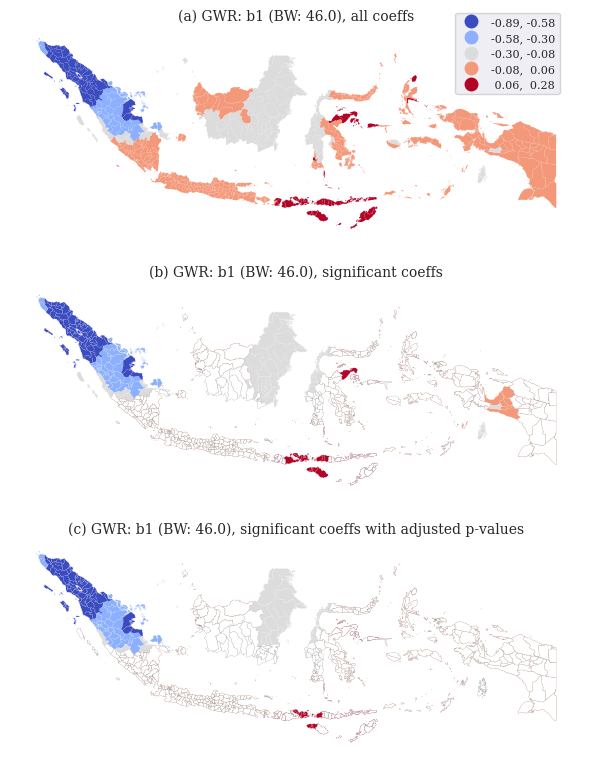
\includegraphics[width=\linewidth]{gwr_b1.png}
        \caption{GWR model: Spatial distribution of the convergence coefficients}
        \label{fig:gwr_b1}
    \end{minipage}

\end{figure}

Based on the code of Application 4, Figure \ref{fig:gwr_b1} shows the spatial distribution of the convergence coefficient.
It presents three progressive visualizations of the GWR convergence coefficient, estimated using a bandwidth of 46 nearest neighbors.
Panel (a) displays the full range of coefficients, with western regions, particularly Sumatra, showing strong convergence (blue shading), while southeastern regions exhibit divergence (red shading), suggesting strong patterns of spatial heterogeneity in regional convergence.
Panels (b) and (c) apply increasingly stringent significance criteria, first using standard significance levels ($\alpha = 0.05$) and then correcting for multiple hypothesis testing. 
This filtering process reveals that while many moderate convergence estimates become statistically insignificant (shown in white color), the strong convergence patterns in western Sumatra and divergence in selected southeastern regions remain robust. 
The persistence of significant coefficients in Sumatra, even after multiple testing correction, underscores the reliability of the convergence process in this region, while suggesting more tentative conclusions about divergence patterns elsewhere.
Overall, the geographic variation in convergence coefficients challenges the assumption of a uniform convergence process across Indonesia. 
The stark contrast between western regions' strong convergence and southeastern areas' potential divergence suggests that national development policies might benefit from geographic differentiation, particularly in addressing the factors driving these distinct regional patterns. 
These findings also point out the value of GWR in revealing spatial nuances that would be masked by global regression approaches.


In a similar way to Application 4, Application 5 shows the spatial distribution the intercept coefficients.
In contrast to non-spatial and spatial dependence models, mapping the intercept is a key component of spatial heterogeneity modeling \citep{Fotheringham2021, mendez2025political, Sachdeva2022}.
The spatial distribution of the intercept help us identify location-specific effects that persist after controlling for covariates. 

\subsubsection*{Application 5: GWR mapping of intercepts}
%  https://colab.research.google.com/drive/1-Q9yPWI0YqwRlsBVlEQ37MDJbljASw30?usp=sharing
% https://bit.ly/MGWRapp5

The code of Application 5 follows a similar structure to Application 4, but focuses on visualizing the spatial distribution of the GWR intercept coefficients ($\beta_0$) rather than the slope coefficients ($\beta_1$). 
It maintains the same three-tiered visualization approach: first mapping all intercept coefficients, then applying standard significance filtering ($\alpha = 0.05$), and finally implementing multiple-testing-corrected p-values. 
The code employs identical cartographic specifications, including the "coolwarm" color scheme, Fisher-Jenks classification, and consistent styling across panels. 
The primary technical difference lies in the indexing of the coefficient arrays, where \texttt{params[:, 0]} selects the intercept coefficients instead of \texttt{params[:, 1]} for the slope coefficients, while maintaining all other visualization parameters and statistical filtering procedures.

\begin{python}
##################################################################
# Application 5: GWR Intercept Mapping and Filtering
# URL: https://bit.ly/MGWRapp5
##################################################################

# 1. Add GWR Intercept Coefficients to the GeoDataFrame
# -------------------------------------
gdf["gwr_intercept"] = gwr_results.params[:, 0]
gdf["gwr_b1"] = gwr_results.params[:, 1]  # Retained for context if needed

# 2. Filter t-values for Significance
# -------------------------------------
# - Standard significance level (alpha = 0.05)
gwr_filtered_t = gwr_results.filter_tvals(alpha=0.05)

# - Adjusted significance level (corrected for multiple testing)
gwr_filtered_tc = gwr_results.filter_tvals()

# 3. Plot the Intercept (b0) Coefficient
# -------------------------------------
fig, axes = plt.subplots(nrows=3, ncols=1, figsize=(12, 8))

# (a) Map of all intercept coefficients
gdf.plot(
    column="gwr_intercept",
    cmap="coolwarm",
    linewidth=0.01,
    scheme="FisherJenks",
    k=5,
    legend=True,
    legend_kwds={"bbox_to_anchor": (0.97, 1.10), "fontsize": 8},
    ax=axes[0]
)

# (b) Map highlighting statistically significant intercept coefficients (alpha = 0.05)
gdf.plot(
    column="gwr_intercept",
    cmap="coolwarm",
    linewidth=0.05,
    scheme="FisherJenks",
    k=5,
    legend=False,
    ax=axes[1]
)
gdf[gwr_filtered_t[:, 0] == 0].plot(
    color="white",
    linewidth=0.05,
    edgecolor="black",
    ax=axes[1]
)

# (c) Map highlighting statistically significant intercept coefficients with adjusted p-values
gdf.plot(
    column="gwr_intercept",
    cmap="coolwarm",
    linewidth=0.05,
    scheme="FisherJenks",
    k=5,
    legend=False,
    ax=axes[2]
)
gdf[gwr_filtered_tc[:, 0] == 0].plot(
    color="white",
    linewidth=0.05,
    edgecolor="black",
    ax=axes[2]
)

# 4. Customize Layout and Appearance
# -------------------------------------
plt.tight_layout()

# Remove axes for a cleaner presentation
for ax in axes:
    ax.axis("off")

# Set subplot titles with consistent styling
axes[0].set_title(
    f"(a) GWR: b0 (BW: {gwr_bw}), all coeffs", fontsize=10
)
axes[1].set_title(
    f"(b) GWR: b0 (BW: {gwr_bw}), significant coeffs", fontsize=10
)
axes[2].set_title(
    f"(c) GWR: b0 (BW: {gwr_bw}), significant coeffs with adjusted p-values",
    fontsize=10
)

# 5. Save and Display the Figure
# -------------------------------------
plt.savefig("gwr_b0.png", dpi=100, bbox_inches="tight")
plt.show()
\end{python}

\begin{figure}[htbp]
    \centering
    \begin{minipage}{0.99\textwidth}
        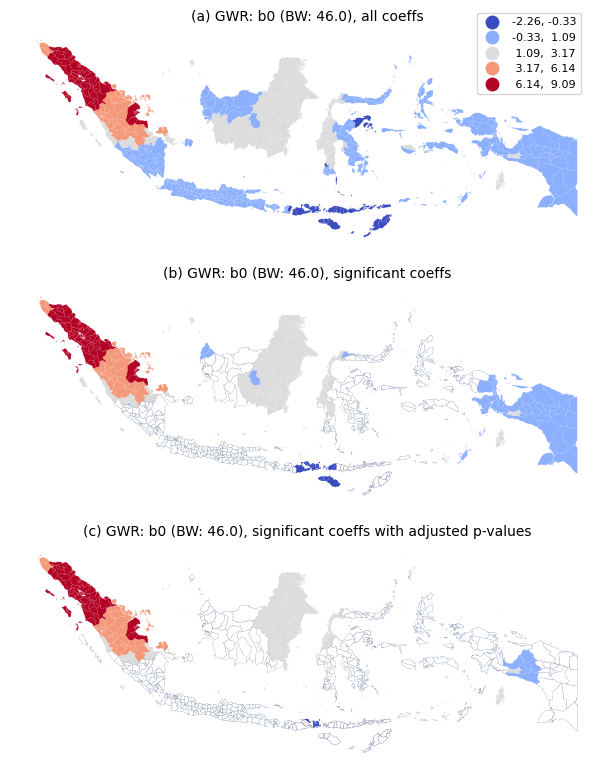
\includegraphics[width=\linewidth]{gwr_b0.png}
        \caption{GWR model: Spatial distribution of the intercepts}
        \label{fig:gwr_b0}
    \end{minipage}
\end{figure}

Based the code of Application 5, Figure \ref{fig:gwr_b1} shows the spatial distribution of the intercept.
In spatial heterogeneity modeling, the intercept term holds particular significance as it captures location-specific effects that persist after controlling for all model covariates. 
The GWR intercept map for Indonesian districts, estimated with a bandwidth of 46 nearest neighbors, reveals distinct spatial clusters in growth patterns. 
The western regions, particularly Sumatra, display significantly positive intercepts, while the rest of Indonesia shows markedly different patterns. 
The progression through significance filters (panels b and c) strengthens our interpretation of these spatial clusters by controlling for both standard significance ($\alpha = 0.05$) and multiple testing. 
The persistence of significant positive intercepts in Sumatra and a few some negative intercepts in select southeastern regions, even after stringent statistical filtering, confirms the presence of  spatial clusters with distinct growth characteristics. 
These clusters likely reflect deep-rooted differences in local economic structures, institutions, and development potential that are not captured by the model's explanatory variables.
As such,  mapping the intercept can reveal important patterns of spatial heterogeneity that might otherwise remain hidden in traditional regression analyses.

\subsubsection{Multiscale geographically weighted regression}


The recognition that different processes operate at different spatial scales represents a fundamental challenge to the original GWR framework. 
While GWR advanced the frontier of spatial analysis by allowing relationships to vary across space, it maintained the restrictive assumption that all relationships vary at the same spatial scale. 
For example, this assumption becomes highly restrictive when examining complex regional phenomena where institutional factors might operate at broad scales while market dynamics function locally. 
Multiscale Geographically Weighted Regression (MGWR) emerges as a new advancement that addresses this limitation of a unique scale by allowing each variable in a model to operate at its own optimal spatial scale.

The practical implications of this methodological advance are profound. 
Consider a regional growth model where infrastructure investment effects might span entire metropolitan regions, educational impacts operate at county levels, and local business climate effects function at neighborhood scales. 
Traditional GWR would force all these relationships to share a single spatial scale (bandwidth), inevitably compromising the accuracy of at least some relationships. 
MGWR liberates the analysis from this constraint, allowing the data to reveal the natural scale at which each process operates. 
This multiscale capability informs our understanding of spatial processes from a single-lens view to a multi-resolution perspective that better reflects the complexity of real-world phenomena.

\subsubsection*{Conceptual foundations and motivation}

The development of MGWR stems from both theoretical considerations and empirical observations that challenged the single-scale assumption of GWR. 
Theoretical work in geography has long recognized that processes operate at different scales—from local interactions to regional systems to global forces \citep{Fotheringham2017}. 
The concept of operational scale, which refers to the spatial extent at which a process manifests its effects, varies naturally across different phenomena.
Climate effects on agriculture might operate at continental scales, while soil quality impacts function at field levels. 
This scale multiplicity cannot be captured by methods that impose a single scale of analysis.

Empirical evidence for scale-specific processes accumulated through GWR applications that produced unsatisfactory results.
The researchers noticed that optimal bandwidths often represented uncomfortable compromises: too large to capture local variations in some relationships, yet too small to provide stable estimation of others. 
\cite{Fotheringham2017} documented cases where forcing all relationships to share a bandwidth led to either over-smoothing of local processes or under-smoothing of regional ones, motivating the development of a more flexible framework.

The intellectual foundation for MGWR draws from the generalized additive model (GAM) literature in statistics \citep{hastie1990generalized}. 
GAMs allow different covariates to have different degrees of smoothness in their relationships with the response variable. 
MGWR adapts this principle to the spatial context, where smoothness translates to spatial scale. 
Each covariate receives its own bandwidth parameter, determining the spatial scale at which that specific process operates. 
This connection to GAMs provides MGWR with a solid statistical foundation while maintaining the geographical intuition of GWR.

\subsubsection*{Practical differences between GWR and MGWR}

The practical distinctions between GWR and MGWR extend beyond the obvious allowance for multiple bandwidths. 
These differences fundamentally alter how analysts approach spatial heterogeneity and interpret results. 
Understanding these distinctions is crucial for practitioners deciding between the two methods and for interpreting MGWR results correctly.

The most immediate practical difference lies in bandwidth optimization. 
GWR employs a single optimization procedure to find one bandwidth that minimizes a global criterion such as AICc. 
Although computationally straightforward, this process forces a compromise (that is, the same spatial scale) in all covariates. 
MGWR, in contrast, employs an iterative backfitting algorithm that optimizes each bandwidth conditional on the others. 
This creates a more complex optimization landscape but yields bandwidths that better reflect the spatial scale of each covariate.
The computational burden increases substantially, but the gain in model realism often justifies this cost.

Model interpretation changes fundamentally between GWR and MGWR. 
In GWR, the single bandwidth provides a general indication of the overall scale of spatial heterogeneity in the system. 
A small bandwidth suggests predominantly local processes, while a large bandwidth indicates that regional or global processes dominate. 
This interpretation, while useful, obscures the potentially rich multiscale nature of the phenomena. 
MGWR produces a vector of bandwidths, each indicating the operational scale of a specific covariate. 
This approach allows us to identify which covariates operate locally and which have broader spatial influence, which critical information for policy design and theoretical understanding.

The interpretation of the parameter surface also differs markedly. 
GWR produces parameter surfaces that all share the same level of spatial smoothness, determined by the global bandwidth. 
This can lead to spuriously detailed variation in relationships that actually operate at broad scales, or overly smooth representations of truly local processes. 
The surfaces of the MGWR parameters exhibit covariate-specific smoothness.
A parameter surface associated with a large bandwidth appears smooth and regional, while one with a small bandwidth shows fine-grained local variation. 
This visual difference immediately communicates the scale at which each process operates.

Standard error surfaces in MGWR provide more realistic uncertainty quantification than GWR. 
Because each relationship uses its appropriate bandwidth, the standard errors reflect the actual information available at the operational scale of each covariate.
Relationships operating at broad scales have more stable estimates with smaller standard errors, while truly local relationships appropriately show higher uncertainty. 
GWR's single bandwidth forces all relationships to have similar uncertainty patterns, potentially understating uncertainty for local processes or overstating it for regional ones.


Hypothesis testing in MGWR accounts for the different scales at which covariates operate.
The multiple testing correction must consider that different parameters have different effective sample sizes based on their bandwidths.
\cite{Yuetal2020} developed parameter-specific inference procedures that account for these scale differences, providing more accurate significance testing than applying uniform corrections across all parameters.

\subsubsection*{Multiple bandwidths and spatial scales}

The interpretation of scale through bandwidths represents perhaps MGWR's most significant contribution to spatial analysis. 
Each optimized bandwidth provides a direct measure of the spatial scale at which a particular covariate operates.
This scale information transcends mere technical parameters to reveal fundamental properties of the processes under study.

The bandwidth magnitude directly indicates the spatial extent of the process operation. 
For an adaptive kernel specified as k-nearest neighbors, the bandwidth represents the number of neighboring observations that significantly influence parameter estimation at each location. 
For example, a small bandwidth of 50 may suggest that the process operates at a local scale, with the estimated coefficients changing over relatively short distances. 
In contrast, a large bandwidth approaching the sample size indicates a global process with little spatial variation. 
Between these extremes, various regional scales emerge, each potentially representing different institutional, economic, or environmental factors.

The relative comparison of bandwidths across covariates reveals the multiscale structure of spatial phenomena. 
In a regional development model, if education effects have a bandwidth of 200 regions, while infrastructure impacts show a bandwidth of 50 regions, this difference suggests education's influence on growth operates at broader regional scales while infrastructure effects remain localized. 
Such scale contrasts provide information on the mechanisms driving spatial patterns and the appropriate level for policy interventions.

Scale interpretation extends to understanding process stationarity. 
\cite{Fotheringham2017} propose that bandwidths approaching the sample size indicate effectively stationary processes that show minimal spatial variation. 
Rather than forcing binary decisions about parameter homogeneity, MGWR provides a continuum where a covariate can be "nearly stationary" with very large bandwidths or "highly local" with small ones. 
This nuanced view better reflects the reality that some processes exhibit subtle spatial variation that might be statistically significant, but practically modest.

Bandwidth uncertainty, often overlooked in GWR applications, becomes crucial for scale interpretation in MGWR. 
\cite{li2020measuring} developed methods to quantify bandwidth uncertainty, showing that some processes have well-defined scales (narrow bandwidth confidence intervals) while others exhibit scale ambiguity (wide intervals). 
This uncertainty information helps distinguish processes with clear operational scales from those with more diffuse spatial influences.

The temporal stability of scales, revealed through repeated MGWR analyses over time, indicates whether process scales are fixed or evolving. 
\cite{wolf2021place} demonstrated that some covariates maintain consistent scales over decades while others show scale evolution, possibly reflecting changing technology, infrastructure, or institutional arrangements. 
This temporal perspective on scale adds another dimension to MGWR interpretation.

\subsubsection*{Mathematical derivation:  A brief overview}

The mathematical formulation of MGWR extends that of the GWR framework by allowing parameter-specific weight matrices. The fundamental model remains:
$$y_i = \sum_{j=0}^{k} \beta_j(u_i, v_i)x_{ij} + \varepsilon_i$$
However, each parameter $\beta_j(u_i, v_i)$ is now estimated using its own spatial weight matrix $\mathbf{W}_i^{(j)}$ determined by bandwidth $b_j$:
$$\hat{\beta}_j(u_i, v_i) = \mathbf{e}_j^T(\mathbf{X}^T\mathbf{W}_i^{(j)}\mathbf{X})^{-1}\mathbf{X}^T\mathbf{W}_i^{(j)}\mathbf{y}$$
where $\mathbf{e}_j$ is a vector selecting the $j$-th parameter.

The key innovation lies in the estimation algorithm. Direct optimization over all bandwidths simultaneously proves computationally intractable and numerically unstable. Instead, MGWR employs a backfitting algorithm inspired by GAM estimation. The algorithm iteratively cycles through parameters, optimizing each bandwidth conditional on current estimates of the others.

The backfitting algorithm proceeds as follows:
\begin{itemize}
    \item Initialize with GWR estimates using a common bandwidth
    \item For each iteration until convergence:
    \begin{itemize}
        \item For each parameter $j = 0, 1, ..., k$:
        \begin{itemize}
            \item Form partial residuals: $r_i^{(j)} = y_i - \sum_{l \neq j} \hat{\beta}_l(u_i, v_i)x_{il}$
            \item Find optimal bandwidth $b_j$ by regressing $r^{(j)}$ on $x_j$ using GWR
            \item Update parameter estimates $\hat{\beta}_j$ using the optimized bandwidth
        \end{itemize}
        \item Check convergence based on parameter stability
    \end{itemize}
\end{itemize}

This algorithm elegantly decomposes the complex multiscale optimization into a series of simpler single-scale problems. Each iteration improves the model fit while respecting the different scales at which processes operate. Convergence typically occurs within 5-15 iterations for well-conditioned problems.

The effective number of parameters in MGWR becomes parameter-specific:
$$ENP_j = \mathrm{tr}(\mathbf{R}_j)$$
where $\mathbf{R}_j$ is the hat matrix component corresponding to parameter $j$. The total model complexity is:
$$ENP_{total} = \sum_{j=0}^{k} ENP_j$$
This decomposition reveals how model complexity is distributed across covariates, with locally varying parameters contributing more to complexity than regional or global ones.

\subsubsection*{Model selection and comparison with GWR}

The model selection framework for MGWR extends beyond simple comparisons with GWR to encompass decisions about which parameters should vary spatially and at what scales. 
The AICc for MGWR accounts for the total effective degrees of freedom:
$$AICc_{MGWR} = 2n\ln(\hat{\sigma}) + n\ln(2\pi) + n\left(\frac{n + \mathrm{tr}(\mathbf{S})}{n - 2 - \mathrm{tr}(\mathbf{S})}\right),$$
where $\mathbf{S} = \sum_{j=0}^{k} \mathbf{R}_j$ is the combined hat matrix.

Comparing MGWR with GWR involves more than examining the AICc values. 
The pattern of bandwidths provides diagnostic information: if all MGWR bandwidths cluster near the single GWR bandwidth, this suggests limited scale heterogeneity and GWR may suffice. 
Conversely, widely varying MGWR bandwidths indicate substantial scale heterogeneity that GWR cannot capture. \cite{Fotheringham2017} suggest bandwidth ratios exceeding 2:1 as indicating meaningful scale differences.

Model building strategies for MGWR differ from traditional approaches. 
Rather than starting with a full model and removing insignificant terms, one might begin with global parameters and selectively allow spatial variation where theoretically justified or empirically supported. 
\cite{comber2020route} propose a systematic approach: first estimate a global model, then GWR, then MGWR, examining at each stage whether added complexity is justified by improved fit and interpretability.

The selection between fixed and spatially varying parameters within MGWR remains an active area of research. 
Parameters with bandwidths approaching the sample size might be candidates for global treatment, simplifying the model and improving interpretability. 
\cite{mei2006testing} developed formal tests for parameter stationarity within the MGWR framework, though these require careful interpretation given the multiple testing issues.

\subsubsection*{Some recent studies illustrating the advantages of MGWR}

The superior performance of MGWR over GWR has been discussed in recent studies.
A common feature of these studies is the revealing of previously hidden multiscale processes. 
These applications not only validate the methodology, but also generate new insights into spatial phenomena.

In urban analytics, \cite{fotheringham2019examining} applied MGWR to housing price determinants in Phoenix, revealing that structural attributes (size, bedrooms) operate at local scales while neighborhood amenities influence prices regionally. 
This multiscale structure was obscured in the GWR analysis, forcing all relationships to share an intermediate bandwidth.
The MGWR results aligned with housing market theory: individual preferences for structural attributes vary locally, while amenity values reflect broader market areas.

Environmental applications have particularly benefited from the multiscale capabilities of MGWR. 
\cite{yang2020exploring} examined air pollution determinants in China, finding that meteorological factors operated on continental scales, while emission sources showed local impacts. 
The scale differences--—bandwidths varying by factors of ten—--could not be accommodated within GWR's single-scale framework. 
These findings informed pollution control strategies by identifying interventions that required regional coordination versus local action.

Public health research has adopted MGWR to understand disease determinants on a wide range of spatial scales. 
\cite{oshan2020targeting} investigated obesity prevalence, discovering that built environment factors operated locally while socioeconomic influences spanned broader areas. 
This scale insight proved crucial for intervention design: physical activity infrastructure requires neighborhood-level planning, while addressing food access might require regional approaches.

Regional convergence studies demonstrate MGWR's ability to reveal scale-dependent processes. 
\cite{murakami2021spatially} reexamined European regional convergence using MGWR, finding that human capital effects operated at national scales while infrastructure impacts remained regional. 
This challenged previous GWR studies suggesting uniform regional effects and highlighted how different convergence mechanisms operate at distinct spatial scales.

Transportation research has used MGWR to understand multiscale mobility patterns. 
\cite{zhang2021multiscale} analyzed factors influencing transit ridership, revealing that employment density effects operated at metropolitan scales while residential density impacts were highly localized. 
These scale differences explained previous inconsistent findings and informed transit planning strategies appropriate to each factor's operational scale.


\subsubsection*{Limitations and caution}

Despite its advantages, MGWR still faces challenges that researchers must consider carefully. 
These limitations do not negate the value of MGWR, but rather define contexts where careful application and interpretation are required.

The curse of dimensionality affects MGWR more severely than GWR. 
With each additional covariate requiring its own bandwidth optimization, the parameter space grows rapidly. 
Models with many covariates may face convergence challenges or produce unstable bandwidth estimates. 
Current practice suggests limiting MGWR to models with fewer than 10-15 covariates, although this depends on sample size and spatial configuration.

Bandwidth interpretation becomes complex when there are strong correlations among covariates. 
Correlated variables may show similar bandwidths not because they operate at the same scale but because the optimization algorithm cannot clearly separate their effects. 
\cite{wheeler2018multicollinearity} demonstrated that multicollinearity can bias bandwidth estimates, suggesting careful variable selection remains important.

Edge effects in MGWR require special consideration. 
Different bandwidths could mean edge effects vary by parameter---the estimated coefficients for some covariates lose precision near boundaries while others remain stable. 
This complicates interpretation in edge regions and may require parameter-specific edge corrections or careful masking of unreliable estimates.

The assumption of smooth parameter variation inherent in the kernel weighting may not suit all applications.
Processes with sharp spatial discontinuities—--such as those at administrative boundaries—--may be poorly represented by smooth kernel functions. 
Recent work on discontinuous MGWR \citep{wang2023discontinuous} begins to address this limitation.

Computational requirements, while improved, still limit very large applications. 
Datasets with hundreds of thousands of observations remain challenging, particularly with many covariates. 
Approximation methods trade accuracy for speed, but optimal trade-offs remain an active research area.


\subsubsection*{Application 6: Estimation of regression coefficients via MGWR}
% https://colab.research.google.com/drive/1Z_0wR17oTNk5gxDRL9yKSBztVCkyRsh0?usp=sharing
% https://bit.ly/MGWRapp6


The code of Application 6 implements a Multiscale Geographically Weighted Regression (MGWR) analysis. 
Although the code shares some similarities with that of Application 5, there are notable differences.
One key difference is the standardization of variables.
This step is essential to ensure the comparability of bandwidths across different covariates.
The code of Application 6 is based on a workflow of six steps: data loading, variable preparation, spatial coordinate extraction, variable standardization, bandwidth selection, and model fitting. 
Each step utilizes specific functions and arguments to transform raw geospatial data into a spatial statistical model capable of revealing location-specific economic relationships.

The initial stages focus on data preparation, where the script loads a GeoJSON file containing Indonesian spatial economic data, extracts the dependent variable (GDP growth) and independent variable (log GDP per capita), and creates coordinate pairs for spatial analysis.
Critical preprocessing steps include standardizing variables by centering them around zero and scaling to unit variance. 
The final stages leverage the \verb|Sel_BW()| function for adaptive bandwidth selection and the \verb|MGWR()| function for model estimation. 
These functions dynamically adjust regression parameters across spatial locations, allowing the model to capture nuanced, locally varying economic relationships.

\begin{python}
##################################################################
# Application 6: Multiscale Geographically Weighted Regression
# URL: https://bit.ly/MGWRapp6
##################################################################

# 1. Load Data
# -------------------------------------
gdf = gpd.read_file(
    "https://github.com/quarcs-lab/data-quarcs/raw/refs/heads/master/"
    "indonesia514/gdfBeta.geojson"
)

# 2. Prepare Variables
# -------------------------------------
# - Dependent Variable: GDP growth ('g')
y = gdf["g"].values.reshape((-1, 1))  # Reshape to column vector

# - Independent Variable: Log GDP per capita (2010)
X = gdf[["ln_gdppc2010"]].values  # Ensure X is 2D

# - Spatial Coordinates: Extract X and Y coordinates
u, v = gdf["COORD_X"], gdf["COORD_Y"]
coords = list(zip(u, v))  # List of (x, y) tuples

# 3. Standardize Variables
# -------------------------------------
Zy = (y - y.mean(axis=0)) / y.std(axis=0)
ZX = (X - X.mean(axis=0)) / X.std(axis=0)

# 4. Select Optimal Bandwidth for MGWR
# -------------------------------------
mgwr_selector = Sel_BW(coords, Zy, ZX, multi=True)
mgwr_bw = mgwr_selector.search()

# 5. Fit the MGWR Model
# -------------------------------------
mgwr_results = MGWR(coords, Zy, ZX, mgwr_selector).fit()

# 6. Display Model Summary
# -------------------------------------
mgwr_results.summary()
\end{python}

\begin{table}[h]
\centering
\caption{Multi-Scale Geographically Weighted Regression (MGWR) Results}
\label{tab:mgwr}
\small
\begin{tabular}{lr}
\hline

\multicolumn{2}{c}{\textbf{Global regression statistics}} \\
\hline
Residual sum of squares & 404.242 \\
Log-likelihood & -667.601 \\
AIC & 1339.202 \\
AICc & 1341.249 \\
BIC & -2791.776 \\
R\textsuperscript{2} & 0.214 \\
Adj. R\textsuperscript{2} & 0.212 \\
\hline

\multicolumn{2}{c}{\textbf{Global regression estimates}} \\
\hline
 & Estimate (SE)  \\
Standardized intercept & -0.000 (0.039)  \\
Standardized convergence coefficient & -0.462 (0.039)$^{***}$  \\
\hline

\multicolumn{2}{c}{\textbf{MGWR bandwidths}} \\
\hline

Standardized intercept & 44.000  \\
Standardized convergence coefficient & 44.000  \\
\hline

\multicolumn{2}{c}{\textbf{Local MGWR regression statistics}} \\
\hline
Residual sum of squares & 122.052 \\
Log-likelihood & -359.826 \\
AIC & 825.783 \\
AICc & 838.259 \\
BIC & 1050.898 \\
R\textsuperscript{2} & 0.763 \\
Adjusted R\textsuperscript{2} & 0.736 \\
Adj. alpha (95\%) for intercept & 0.002 \\
Adj. alpha (95\%) for convergence coefficient & 0.002 \\
\hline

\multicolumn{2}{c}{\textbf{Local MGWR regression estimates}} \\
\hline
 & Mean (STD) [Min, Median, Max] \\
Standardized intercept & 0.023 (0.276) [-0.487, -0.048, 1.185] \\
Standardized convergence coefficient & -0.313 (0.553) [-1.744, -0.084, 0.417] \\
\hline
\multicolumn{2}{l}{\textit{Note:} $***p<0.001$} \\
\end{tabular}
\end{table}

Based on the code of Application 6, Table \ref{tab:mgwr} shows the results of the MGWR model. 
For comparison and benchmark purposes, Table \ref{tab:mgwr} also shows the results of a standard/global OLS model at the top. 
The global regression results establish a baseline for understanding regional growth dynamics in Indonesian districts, revealing a significant (standardized) convergence coefficient ($\beta = -0.462$, $p<0.001$) but modest explanatory power ($R^2 = 0.214$). 
This limited fit of the global model suggests substantial unexplained variation in growth patterns, motivating the exploration of spatial heterogeneity.

The MGWR specification shows substantially improved explanatory power, with $R^2$ increasing to 0.763 (adjusted $R^2 = 0.736$) and notable improvements in model selection criteria (AIC decreases from 1339.202 to 825.783; RSS reduces from 404.242 to 122.052). 
This enhancement in model fit indicates that spatial heterogeneity plays a crucial role in explaining regional growth variations across Indonesian districts.
An interesting finding is that both regression parameters share the same optimal bandwidth ($bw = 44$), indicating that baseline growth patterns and convergence dynamics operate at similar spatial scales of 44 neighbors. 
This consistent spatial scale, identified through the MGWR framework's optimization algorithm, highlights the geographic extent of regional growth processes. 


The local parameter estimates reveal substantial spatial heterogeneity in both the intercept ($\beta_0 \in [-0.487, 1.185]$) and convergence coefficient ($\beta_1 \in [-1.744, 0.417]$). 
The median convergence coefficient ($\beta_{1,median} = -0.084$) differs notably from the global estimate, indicating that some regions exhibit strong convergence while others show evidence of divergence. 
These findings have important implications for regional development policy in Indonesia, suggesting that uniform national development strategies may be suboptimal. 
The identification of distinct convergence patterns, operating at a consistent spatial scale, indicates that policy interventions should be tailored to local conditions while considering the characteristic spatial extent of growth processes.


In addition to tabular results, presenting the findings through choropleth maps can provide more informative and persuasive insights.
In Application 7, the spatial distribution of the convergence coefficients from the MGWR model is presented.
A crucial aspect of this visualization is the acknowledgment that the convergence coefficient is not statistically significant in all regions.
Filtering out regions with non-significant coefficients is a key feature of spatial heterogeneity modeling.


\subsubsection*{Application 7: MGWR mapping of convergence coefficients}
% https://colab.research.google.com/drive/1FhWJoPwODIG7yYsyFUwn5qGF4TLHreLi?usp=sharing
% https://bit.ly/MGWRapp7

The code of Application 7 a structured five-step process for visualizing Multiscale Geographically Weighted Regression (MGWR) results, closely mirroring the approach of Application 4. 
It begins by extracting model coefficients into the geospatial data frame, then applies statistical significance filtering at standard and adjusted levels. 
Using matplotlib, the script creates three subplots that progressively reveal spatial variations: a baseline map of all coefficients, a map highlighting statistically significant coefficients at $\alpha = 0.05$, and a third map with coefficients significant after p-value correction due to multiple testing.
Employing techniques like Fisher-Jenks classification and color mapping, the visualization systematically transforms complex statistical data into an intuitive geographical representation. 
The final stage focuses on aesthetic refinement, removing axes, adding informative titles with bandwidth details, and saving the figure.

\begin{python}
##################################################################
# Application 7: MGWR mapping of convergence coefficients
# URL: https://bit.ly/MGWRapp7
##################################################################

# 1. Add MGWR Coefficients to the GeoDataFrame
# -------------------------------------
gdf["mgwr_intercept"] = mgwr_results.params[:, 0]
gdf["mgwr_b1"] = mgwr_results.params[:, 1]

# 2. Filter t-values for Significance
# -------------------------------------
# - Standard significance level (alpha = 0.05)
mgwr_filtered_t = mgwr_results.filter_tvals(alpha=0.05)

# - Adjusted significance level (corrected for multiple testing)
mgwr_filtered_tc = mgwr_results.filter_tvals()

# 3. Plot the b1 Coefficient
# -------------------------------------
fig, axes = plt.subplots(nrows=3, ncols=1, figsize=(12, 8))

# (a) Map of all b1 coefficients
gdf.plot(
    column="mgwr_b1",
    cmap="coolwarm",
    linewidth=0.01,
    scheme="FisherJenks",
    k=5,
    legend=True,
    legend_kwds={"bbox_to_anchor": (0.97, 1.10), "fontsize": 8},
    ax=axes[0]
)

# (b) Map highlighting statistically significant b1 coefficients (alpha = 0.05)
gdf.plot(
    column="mgwr_b1",
    cmap="coolwarm",
    linewidth=0.05,
    scheme="FisherJenks",
    k=5,
    legend=False,
    ax=axes[1]
)
gdf[mgwr_filtered_t[:, 1] == 0].plot(
    color="white",
    linewidth=0.05,
    edgecolor="black",
    ax=axes[1]
)

# (c) Map highlighting b1 coefficients with adjusted p-values
gdf.plot(
    column="mgwr_b1",
    cmap="coolwarm",
    linewidth=0.05,
    scheme="FisherJenks",
    k=5,
    legend=False,
    ax=axes[2]
)
gdf[mgwr_filtered_tc[:, 1] == 0].plot(
    color="white",
    linewidth=0.05,
    edgecolor="black",
    ax=axes[2]
)

# 4. Customize Layout and Appearance
# -------------------------------------
plt.tight_layout()

# Remove axes for a cleaner presentation
for ax in axes:
    ax.axis("off")

# Set subplot titles with consistent styling
axes[0].set_title(
    f"(a) MGWR: b1 (BW: {mgwr_bw[1]}), all coeffs", fontsize=10
)
axes[1].set_title(
    f"(b) MGWR: b1 (BW: {mgwr_bw[1]}), significant coeffs", fontsize=10
)
axes[2].set_title(
    f"(c) MGWR: b1 (BW: {mgwr_bw[1]}), significant coeffs and corr. p-values",
    fontsize=10
)

# 5. Save and Display the Figure
# -------------------------------------
plt.savefig("mgwr_b1.png", dpi=100, bbox_inches="tight")
plt.show()
\end{python}

\begin{figure}[htbp]
    \centering
    \begin{minipage}{0.99\textwidth}
        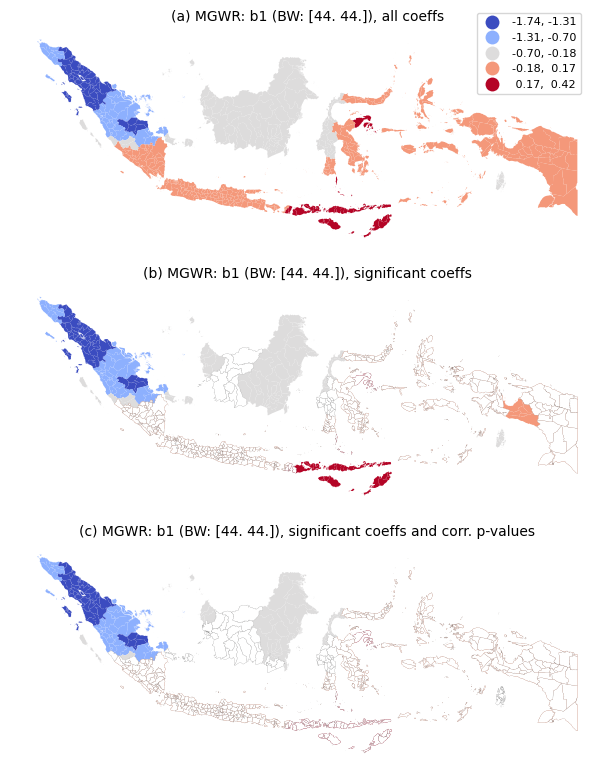
\includegraphics[width=\linewidth]{mgwr_b1.png}
        \caption{MGWR model: Spatial distribution of the intercepts}
        \label{fig:mgwr_b1}
    \end{minipage}
\end{figure}

The MGWR results of Figure \ref{fig:mgwr_b1} reveals the patterns of spatial heterogeneity the process of regional convergence across Indonesian districts. 
Strong convergence (indicated by dark blue coefficients) is concentrated in Sumatra in the western region, suggesting that initially poor districts are catching up with richer ones. 
In contrast, divergence patterns (shown in dark red) are observed in south eastern regions, particularly Nusa Tenggara, indicating a widening income gap between rich and poor districts. 

When evaluating statistical significance in panels (b) and (c), many regions show insignificant convergence/divergence patterns, though Sumatra's convergence process remain robust. 
This filtering of statistically significant coefficients helps identify where the convergence/divergence processes are most reliable. 
The persistence of significant patterns in certain regions suggests localized structural factors driving regional inequality.

The bandwidth of 44 districts in the MGWR model indicates that convergence processes operate at a regional rather than national scale. 
This relatively local bandwidth suggests that economic spillovers and growth processes are geographically bounded, potentially due to infrastructure connectivity, institutional similarities, or cultural ties within regions. 

The identification of spatial heterogeneity patterns may inform the formulation of regional development policies.
For instance, the variation in convergence patterns suggests that uniform national development policies may be ineffective. 
Instead, targeted interventions may be needed, particularly in diverging eastern regions. 
Meanwhile, Sumatra's successful convergence patterns could provide valuable policy lessons for other regions. 
The MGWR analysis thus reveals local processes that would be masked by traditional global regression approaches, highlighting the importance of considering local variations in economic development.


In a similar way to Application 7, Application 8 shows the spatial distribution the intercept coefficients.
In contrast to non-spatial and spatial dependence models, mapping the intercept is a key component of spatial heterogeneity modeling \citep{Fotheringham2021, mendez2025political, Sachdeva2022}.
The spatial distribution of the intercept help us identify location-specific effects that persist after controlling for covariates. 

\subsubsection*{Application 8: MGWR mapping of intercepts}
% https://colab.research.google.com/drive/1gGvI36bdMK7BO8XhxaS1G2TiBe17wAlA?usp=sharing
% https://bit.ly/MGWRapp8

Similar to Application 5, the code of Application 8 presents the spatial distribution of the intercept coefficients.
The code follows a similar sequential structure: first, it adds MGWR intercept coefficients to a GeoDataFrame containing spatial data. 
It then applies two types of significance filtering---one using standard significance levels ($\alpha =0.05$) and another using adjusted p-values that correct for multiple testing. 
The visualization component creates a three-panel figure: the top panel shows all intercept coefficients, the middle panel displays only statistically significant coefficients at the standard significance level, and the bottom panel shows coefficients significant after multiple testing adjustment. 
Each map uses Fisher-Jenks classification for optimal data breaks, and non-significant districts are masked in white. 
The code concludes with layout customization and figure export. 

\begin{python}
##################################################################
# Application 8: MGWR mapping of intercepts
# URL: https://bit.ly/MGWRapp8
##################################################################

# 1. Add MGWR Intercept Coefficients to the GeoDataFrame
# -------------------------------------
gdf["mgwr_intercept"] = mgwr_results.params[:, 0]
gdf["mgwr_b1"] = mgwr_results.params[:, 1]  # Retained for context if needed

# 2. Filter t-values for Significance
# -------------------------------------
# - Standard significance level (alpha = 0.05)
mgwr_filtered_t = mgwr_results.filter_tvals(alpha=0.05)
# - Adjusted significance level (corrected for multiple testing)
mgwr_filtered_tc = mgwr_results.filter_tvals()

# 3. Plot the Intercept (b0) Coefficient
# -------------------------------------
fig, axes = plt.subplots(nrows=3, ncols=1, figsize=(12, 8))

# (a) Map of all intercept coefficients
gdf.plot(
    column="mgwr_intercept",
    cmap="coolwarm",
    linewidth=0.01,
    scheme="FisherJenks",
    k=5,
    legend=True,
    legend_kwds={"bbox_to_anchor": (0.97, 1.10), "fontsize": 8},
    ax=axes[0]
)

# (b) Map highlighting statistically significant intercept coefficients (alpha = 0.05)
gdf.plot(
    column="mgwr_intercept",
    cmap="coolwarm",
    linewidth=0.05,
    scheme="FisherJenks",
    k=5,
    legend=False,
    ax=axes[1]
)
gdf[mgwr_filtered_t[:, 0] == 0].plot(
    color="white",
    linewidth=0.05,
    edgecolor="black",
    ax=axes[1]
)

# (c) Map highlighting intercept coefficients with adjusted p-values
gdf.plot(
    column="mgwr_intercept",
    cmap="coolwarm",
    linewidth=0.05,
    scheme="FisherJenks",
    k=5,
    legend=False,
    ax=axes[2]
)
gdf[mgwr_filtered_tc[:, 0] == 0].plot(
    color="white",
    linewidth=0.05,
    edgecolor="black",
    ax=axes[2]
)

# 4. Customize Layout and Appearance
# -------------------------------------
plt.tight_layout()
for ax in axes:
    ax.axis("off")

axes[0].set_title(f"(a) MGWR: b0 (BW: {mgwr_bw[0]}), all coeffs", fontsize=10)
axes[1].set_title(f"(b) MGWR: b0 (BW: {mgwr_bw[0]}), significant coeffs", fontsize=10)
axes[2].set_title(f"(c) MGWR: b0 (BW: {mgwr_bw[0]}), significant coeffs and corr. p-values", fontsize=10)

# 5. Save and Display the Figure
# -------------------------------------
plt.savefig("mgwr_b0.png", dpi=100, bbox_inches="tight")
plt.show()    
\end{python}

\begin{figure}[htbp]
    \centering
    \begin{minipage}{0.99\textwidth}
        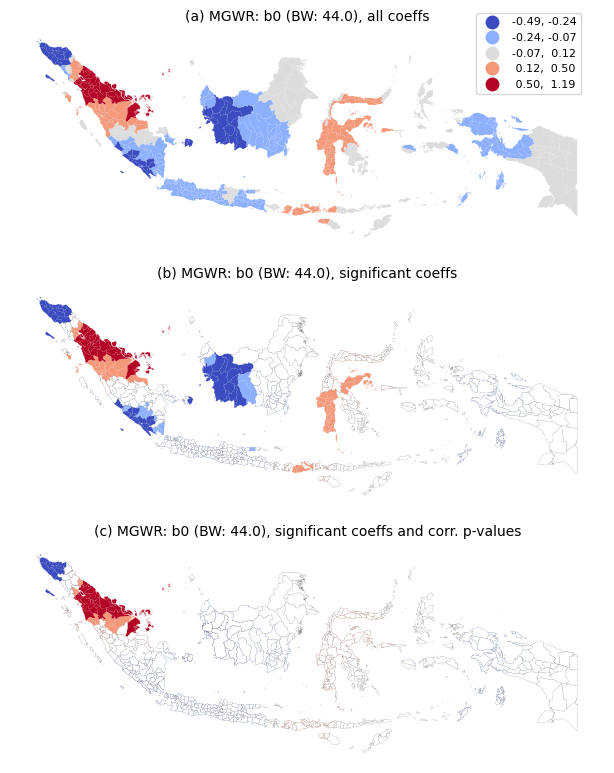
\includegraphics[width=\linewidth]{mgwr_b0.png}
        \caption{MGWR model: Spatial distribution of the intercepts}
        \label{fig:mgwr_b0}
    \end{minipage}
\end{figure}

As in the GWR case,  the intercept term of a MGWR regression  holds special interpretation as it captures location-specific effects that persist after controlling for all model covariates. 
In the context of regional growth studies, these intercepts may represent the underlying growth rates that are unique to each location, independent of the convergence process and other explanatory variables. 
The spatial variation in the intercept could reveal geographic patterns in economic performance that are driven by local characteristics such as infrastructure, institutions, or natural advantages.

The MGWR results for Indonesia (Figure \ref{fig:mgwr_b0}), estimated using 44 nearest neighbors (compared to 46 in the GWR model), show distinct geographical clusters.
Northern Sumatra exhibits strongly positive intercepts (0.50-1.19), indicating areas with persistently higher growth rates independent of the convergence process. 
In contrast, parts of Kalimantan show negative intercepts (-0.49 to -0.24), suggesting systematically lower growth rates.

When examining statistical significance in panels (b) and (c), some of these patterns remain robust, particularly in Sumatra.
The tighter bandwidth of 44 districts suggests these local growth processes operate at a slightly more localized scale than that reported in the GWR analysis (Figure \ref{fig:gwr_b0}).
These findings reinforce the importance of place-based development policies that account for underlying spatial variations in growth dynamics, as areas maintain consistently different growth trajectories regardless of their initial economic conditions.



\section{Concluding remarks}

This chapter introduces the advantages of spatial heterogeneity modeling through the GWR and MGWR frameworks. 
The methodological improvements of these modeling frameworks are substantial.
For example, in our case study application, the R-squared values increased from 0.21 in traditional regression to 0.76 in both GWR and MGWR models. 
Furthermore, a key characteristic of these spatial heterogeneity frameworks is that they are able to differentiate between intrinsic contextual effects (captured by local intercepts) and behavioral contextual effects (shown through spatially varying coefficients).

The distinctive contribution of MGWR lies in its ability to identify specific spatial scales for each covariate and the intercept.
In the Indonesian case study, both the intercept and the convergence coefficient operated at similar scales (44-46 nearest neighbors), suggesting a relatively consistent spatial scale for regional growth processes. 
The spatial scale (bandwidth) represents the optimal number of neighboring regions that should be included in local regression estimates---too few neighbors would increase parameter uncertainty, while too many would introduce bias from dissimilar regions. 
This spatial scale insight is crucial for policy design, as it suggests the geographical extent to which regional development initiatives might be most effective.

Future research directions point toward three key methodological advances: time-varying extensions to MGWR for temporal analysis, integration with machine learning techniques for improved prediction while maintaining interpretability, and extensions to handle non-Gaussian outcomes. 
These developments would broaden the applicability of spatial heterogeneity modeling across different domains while maintaining its core strength in revealing local variations that global models might mask.
The integration of these methods with advanced computational frameworks and cloud computing platforms such as Google Colab will further enhance their accessibility and reproducibility, enabling wider adoption of spatial heterogeneity modeling in regional studies.





%\begin{acknowledgements}
%This work is supported by ...
%\end{acknowledgements}

% BibTeX users please use one of
\bibliographystyle{apalike}    
%\bibliographystyle{spbasic}      % basic style, author-year citations
%\bibliographystyle{spmpsci}      % mathematics and physical sciences
%\bibliographystyle{spphys}       % APS-like style for physics
\bibliography{references}   % name your BibTeX data basehttps://www.overleaf.com/project/5f2d5b386027800001dc941f

% Non-BibTeX users please use
%\begin{thebibliography}{}
%
% and use \bibitem to create references. Consult the Instructions
% for authors for reference list style.
%
%\bibitem{RefJ}
% Format for Journal Reference
%Author, Article title, Journal, Volume, page numbers (year)
% Format for books
%\bibitem{RefB}
%Author, Book title, page numbers. Publisher, place (year)
% etc
%\end{thebibliography}

\newpage

\section*{Appendix}

\section*{Appendix 1: Links to computational notebooks}

\begin{itemize}
    \item \href{https://colab.research.google.com/drive/1Bsr20h4SX9F8TNiaLNO5eHNF5GI5jdps?usp=sharing}{Application 1: Regional growth and convergence in Indonesia \\ https://bit.ly/MGWRapp1}
    \item \href{https://bit.ly/MGWRapp2}{Application 2: Mapping the spatial distribution of initial GDP and growth \\ https://bit.ly/MGWRapp2}
    \item \href{https://bit.ly/MGWRapp3}{Application 3: Estimation of regression coefficients via GWR \\ https://bit.ly/MGWRapp3 }
    \item \href{https://bit.ly/MGWRapp4}{Application 4: GWR mapping of convergence coefficients \\ https://bit.ly/MGWRapp4}
    \item \href{https://bit.ly/MGWRapp5}{Application 5: GWR mapping of intercepts \\ https://bit.ly/MGWRapp5}
    \item \href{https://bit.ly/MGWRapp6}{Application 6: Estimation of regression coefficients via MGWR \\ https://bit.ly/MGWRapp6}
    \item \href{https://bit.ly/MGWRapp7}{Application 7: MGWR mapping of convergence coefficients \\ https://bit.ly/MGWRapp7}
    \item \href{https://bit.ly/MGWRapp8}{Application 8: MGWR mapping of intercepts \\ https://bit.ly/MGWRapp8}
\end{itemize}

\newpage

\section*{Appendix B: List of Python libraries used in this chapter}

\begin{python}
# Adding necessary libraries to Google Colab environment

# Installing the 'contextily' library for adding basemaps
# to plots. This library is useful for adding contextual
# geographical layers, such as maps, to visualizations.
# The '-q' flag is used to suppress unnecessary output.
!pip install contextily -q

# Installing the 'splot' library for spatial data
# visualization. 'splot' works with PySAL to visualize
# spatial data, including spatial autocorrelation and
# cluster analysis. The '-q' flag is used to keep the
# output concise.
!pip install splot -q

# Installing additional libraries for spatial analysis and
# visualization. 'mapclassify' provides classification
# schemes for choropleth mapping, which can be useful for
# grouping spatial data into classes. This helps to
# visualize variations across different spatial regions
# more effectively.
!pip install mapclassify -q  

# Installing the 'mgwr' library for performing
# geographically weighted regression (GWR). GWR is useful
# for understanding spatially varying relationships between
# variables by estimating local regression models. The '-q'
# flag is used to reduce verbosity during installation.
!pip install mgwr -q

# Installing the 'stargazer' library. 'stargazer' is used
# to generate formatted regression tables in a style
# similar to the 'stargazer' R package. This is useful for
# presenting regression results in a well-formatted manner.
# Again, the '-q' flag is used to suppress extra details.
!pip install stargazer -q
\end{python}

\newpage



\end{document}
% end of file template.tex

